\documentclass{../bredelebeamer}
\usepackage{multirow}
\usepackage{pdfpages}
\usepackage{braket,bigstrut}
\usepackage{palatino}
\usepackage{multicol,bigstrut}
\usepackage{listings}
% Tema escogido en este ejemplo

% Velos
\newtheorem{teo}{Teorema}
\newtheorem{ejemplo}{Ejemplo}
\newtheorem{defi}{Definición}
\newtheorem{coro}{Corolario}
\newtheorem{prueba}{Prueba}
\usepackage{tikz}
\usepackage{booktabs}
\usepackage{amsmath,amssymb,amsfonts,cancel}
\usetikzlibrary{positioning,shadows,backgrounds,calc}%
\def\Bb{{\bf{B}}}
\def\Db{{\bf{D}}}
\def\Eb{{\bf{E}}}
\def\Fb{{\bf{F}}}
\def\Kb{{\bf{k}}}
\def\Pb{{\bf{P}}}
\def\ab{{\bf a}}
\def\ib{{\bf{i}}}
\def\jb{{\bf{j}}}
\def\kb{{\bf{k}}}
\def\rb{{\bf r}}
\def\vb{{\bf v}}
\def\entonces{\;\;\;\Longrightarrow\;\;\;}
\newcommand{\der}[3][2]{\frac{d\! #2}{d\! #3}}
\newcommand{\ders}[3][2]{\frac{d^2\! #2}{d\! #3^2}}
\newcommand{\dert}[3][2]{\frac{d^3\! #2}{d\! #3^3}}
\newcommand{\derf}[3][2]{\frac{d^4\! #2}{d\! #3^4}}
\newcommand{\dern}[3][2]{\frac{d^n\! #2}{d\! #3^n}}
\newcommand{\dpr}[3][2]{\frac{\partial #2}{\partial #3}}
\newcommand{\dprs}[3][2]{\frac{\partial^2\! #2}{\partial #3^2}}
\newcommand{\dprt}[3][2]{\frac{\partial^3\! #2}{\partial\! #3^3}}
\newcommand{\dprf}[3][2]{\frac{\partial^4\! #2}{\partial\! #3^4}}
\newcommand{\dprn}[3][2]{\frac{\partial^n\! #2}{\partial\! #3^n}}
\newcommand{\dfr}[3][2]{\frac{\delta\! #2}{\delta\! #3}}
\newcommand{\dfrs}[3][2]{\frac{\delta^2\! #2}{\delta\! #3^2}}
\newcommand{\dfrt}[3][2]{\frac{\delta^3\! #2}{\delta\! #3^3}}
\newcommand{\dfrf}[3][2]{\frac{\delta^4\! #2}{\delta\! #3^4}}
\newcommand{\dfrn}[3][2]{\frac{\delta^n\! #2}{\delta\! #3^n}}
\newcommand{\abs}[1]{\left\vert#1\vphantom{y}\right\vert}%
\newcommand{\eva}[1]{\left.#1\vphantom{\frac yy}\right\vert}%
\newcommand{\cor}[1]{\left[ #1\vphantom{ y}\right]}
\newcommand{\fac}[1]{\left( #1\vphantom{y}\right)}


\setbeamercolor{footnote mark}{fg=black}
\setbeamercolor{footnote}{fg=black}


\renewcommand{\baselinestretch}{0.9}
\title[]{On the sensitivity reach of vector leptoquark production with preferential couplings to third generation fermions at the LHC}
\subtitle{}
\author[Cristian F. Rodríguez]{
	$ $\\
	Cristian Fernando Rodríguez Cruz\\
	$ $\\
	$ $\\
	Authors:\\
	A. Flórez\inst{1}, \textcolor{Framableu}{\textbf{C. Rodriguez}}\inst{1}, J. Peñuela-Parra\inst{1},\\
	J. Jones-Pérez\inst{2}, \\
	A. Gurrola\inst{3},
}

\institute[Uniandes]{\inst{1} Universidad de los Andes\and
\inst{2} Pontificia Universidad Católica del Perú \and 
\inst{3} Vanderbilt University
}
\date{\today}
\lstset{language=C++,
  basicstyle=\ttfamily,
  keywordstyle=\color{blue}\ttfamily,
  stringstyle=\color{red}\ttfamily,
  commentstyle=\color{green}\ttfamily,
  morecomment=[l][\color{magenta}]{\#}
}
\usepackage[backend=bibtex8,style=authortitle,autocite=footnote]{biblatex}
\addbibresource{referencias.bib}

\renewbibmacro*{cite:title}{%
	\printtext[bibhyperref]{%
		\printfield[citetitle]{labeltitle}%
		\setunit{\space}%
		\printtext[parens]{\printdate}%
	}%
}

\renewcommand{\figurename}{{\bf Fig.}}
\usefonttheme{serif} % default family is serif
\newcommand{\PR}{{\pmb{P}_R}}

\newcommand{\PL}{{\pmb{P}_L}}
\definecolor{colordominante}{RGB}{11,17,79}
\definecolor{colordominanteF}{RGB}{219,68,14}
\definecolor{colorejemplo}{RGB}{77,190,208}
\definecolor{colordefinicion}{RGB}{0,51,102}
\definecolor{colorenfermedades}{RGB}{247,252,37}
\definecolor{colorteorema}{RGB}{0,133,202}
\definecolor{colortitulo}{RGB}{0,133,202}
\definecolor{colorcaja}{RGB}{230,050,030}
\definecolor{colorcajas}{RGB}{230,050,030}
\definecolor{grisamarillo}{RGB}{248,248,245} 
\definecolor{amarilloD}{RGB}{251,237,121}
\colorlet{colorfondoejemplo}{gray!10}
\colorlet{colorfondodefinicion}{gray!10}
\colorlet{colorfondoteorema}{gray!10}
\definecolor{colorfondocaja}{RGB}{252,252,244}

\definecolor{rosado}{RGB}{201,148,199}
\definecolor{violeta}{RGB}{117,107,177}
\definecolor{amarilloS}{RGB}{252,252,244}
\definecolor{azulF}{rgb}{.0,.0,.3}
\definecolor{grisD}{rgb}{.3,.3,.3}
\definecolor{grisF}{rgb}{.6,.6,.6}
\definecolor{miverde}{RGB}{44,162,67}
\usetikzlibrary{%
	matrix,
    decorations.pathreplacing,%
    decorations.pathmorphing,%
    decorations.markings,
    arrows,
    fadings,
%   arrows.meta,
    positioning,
    shapes,
    shadows,
    shapes.geometric
    }
		\usepackage{siunitx}
\definecolor{azulF}{rgb}{.0,.0,.3}
\definecolor{myblue1}{RGB}{0,157,209}
\definecolor{myblue2}{RGB}{161,224,255}
\definecolor{myblue3}{RGB}{216,229,245}
\definecolor{myblue4}{RGB}{0,149,229}

\tikzset{
  load/.style={
    ultra thick,
    -latex
  },  
  stress/.style={-latex},
 dim/.style={latex-latex},
  axis/.style={-latex,black!55},
  %
  startstop/.style={
    rectangle, 
    rounded corners=15pt, 
    minimum width=8cm, 
    minimum height=1cm,
    text centered, 
	font=\color{azulF}\sffamily, 
	fill=colorfondodefinicion!70!,
    line width=1pt,
    draw=colorejemplo!65!, 
  },  
 io/.style={
   trapezium, 
   trapezium left angle=70, 
   trapezium right angle=110, 
   minimum width=4cm, 
   minimum height=1cm, 
   text centered, 
	font=\color{azulF}\sffamily, 
	fill=colorfondodefinicion!70!,
    line width=1pt,
    draw=colorejemplo!65!, 
 },  
  process/.style={
    rectangle, 
     rounded corners, 
    minimum width=6cm, 
    minimum height=1cm, 
    text centered, 
    text width=6cm, 
	font=\color{azulF}\sffamily, 
	fill=colorfondodefinicion!70!,
    line width=1pt,
    draw=colorejemplo!65!, 
  },  
    process2/.style={
    rectangle, 
     rounded corners, 
    minimum width=5cm, 
    minimum height=1cm, 
    text centered, 
    text width=5cm, 
	font=\color{azulF}\sffamily, 
	fill=colorfondodefinicion!70!,
    line width=1pt,
    draw=colorejemplo!65!, 
  },     process3/.style={
    rectangle, 
     rounded corners, 
    minimum width=2cm, 
    minimum height=1cm, 
    text centered, 
    text width=2cm, 
	font=\color{azulF}\sffamily, 
	fill=colorfondodefinicion!70!,
    line width=1pt,
    draw=colorejemplo!65!, 
  },  
  decision/.style={
    diamond, 
    minimum width=2.5cm, 
    minimum height=1cm, 
    text width=2.5cm, 
    text centered, 
	font=\color{azulF}\sffamily, 
	fill=colorfondodefinicion!70!,
    line width=1pt,
    draw=colorejemplo!65!, 
  },  
     ragged border/.style={ decoration={random steps, segment length=1mm, amplitude=0.5mm},
           decorate,
   },
}
 \tikzstyle{arrow} = [thick,
    azulF,
    ->,
    >=stealth]
   \tikzfading[name=fade out,
  inner color=transparent!0, outer color=transparent!100]
  \tikzstyle arrowstyle=[scale=1]
\tikzstyle directed=[postaction={decorate,decoration={markings,
    mark=at position .65 with {\arrow[arrowstyle]{stealth}}}}]
\tikzstyle reverse directed=[postaction={decorate,decoration={markings,
    mark=at position .65 with {\arrowreversed[arrowstyle]{stealth};}}}]

\begin{document}

\frame{\titlepage}
% \begin{frame}$ $
%   \begin{small}
%       \tableofcontents
%   \end{small}
% \end{frame}
%\frame{\tableofcontents}


\begin{frame}{Lepton Flavor Universality in the SM of Particle Physics}{What is it?}
	\begin{center}
		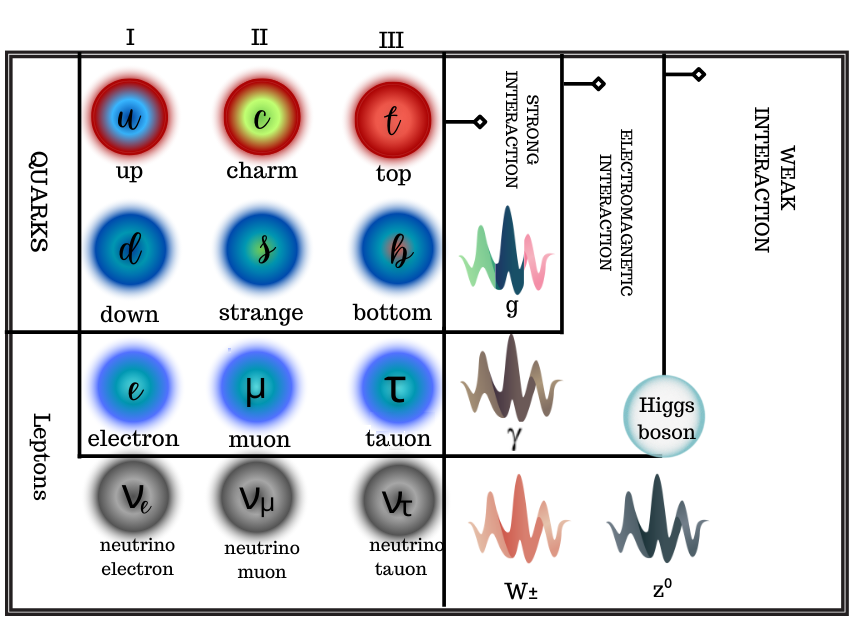
\includegraphics[width=.75\linewidth]{SM.png}	
	\end{center}
	  Weak bosons mix the different generations of quarks via the CKM matrix, but this does not happen for leptons. This property of the model is known as lepton flavor universality (LFU).
 \end{frame}



\begin{frame}{A Hint on Lepton Flavor Universality Violation}{$R(D)$ and $R(D^*)$ anomalies}
	\begin{center}
		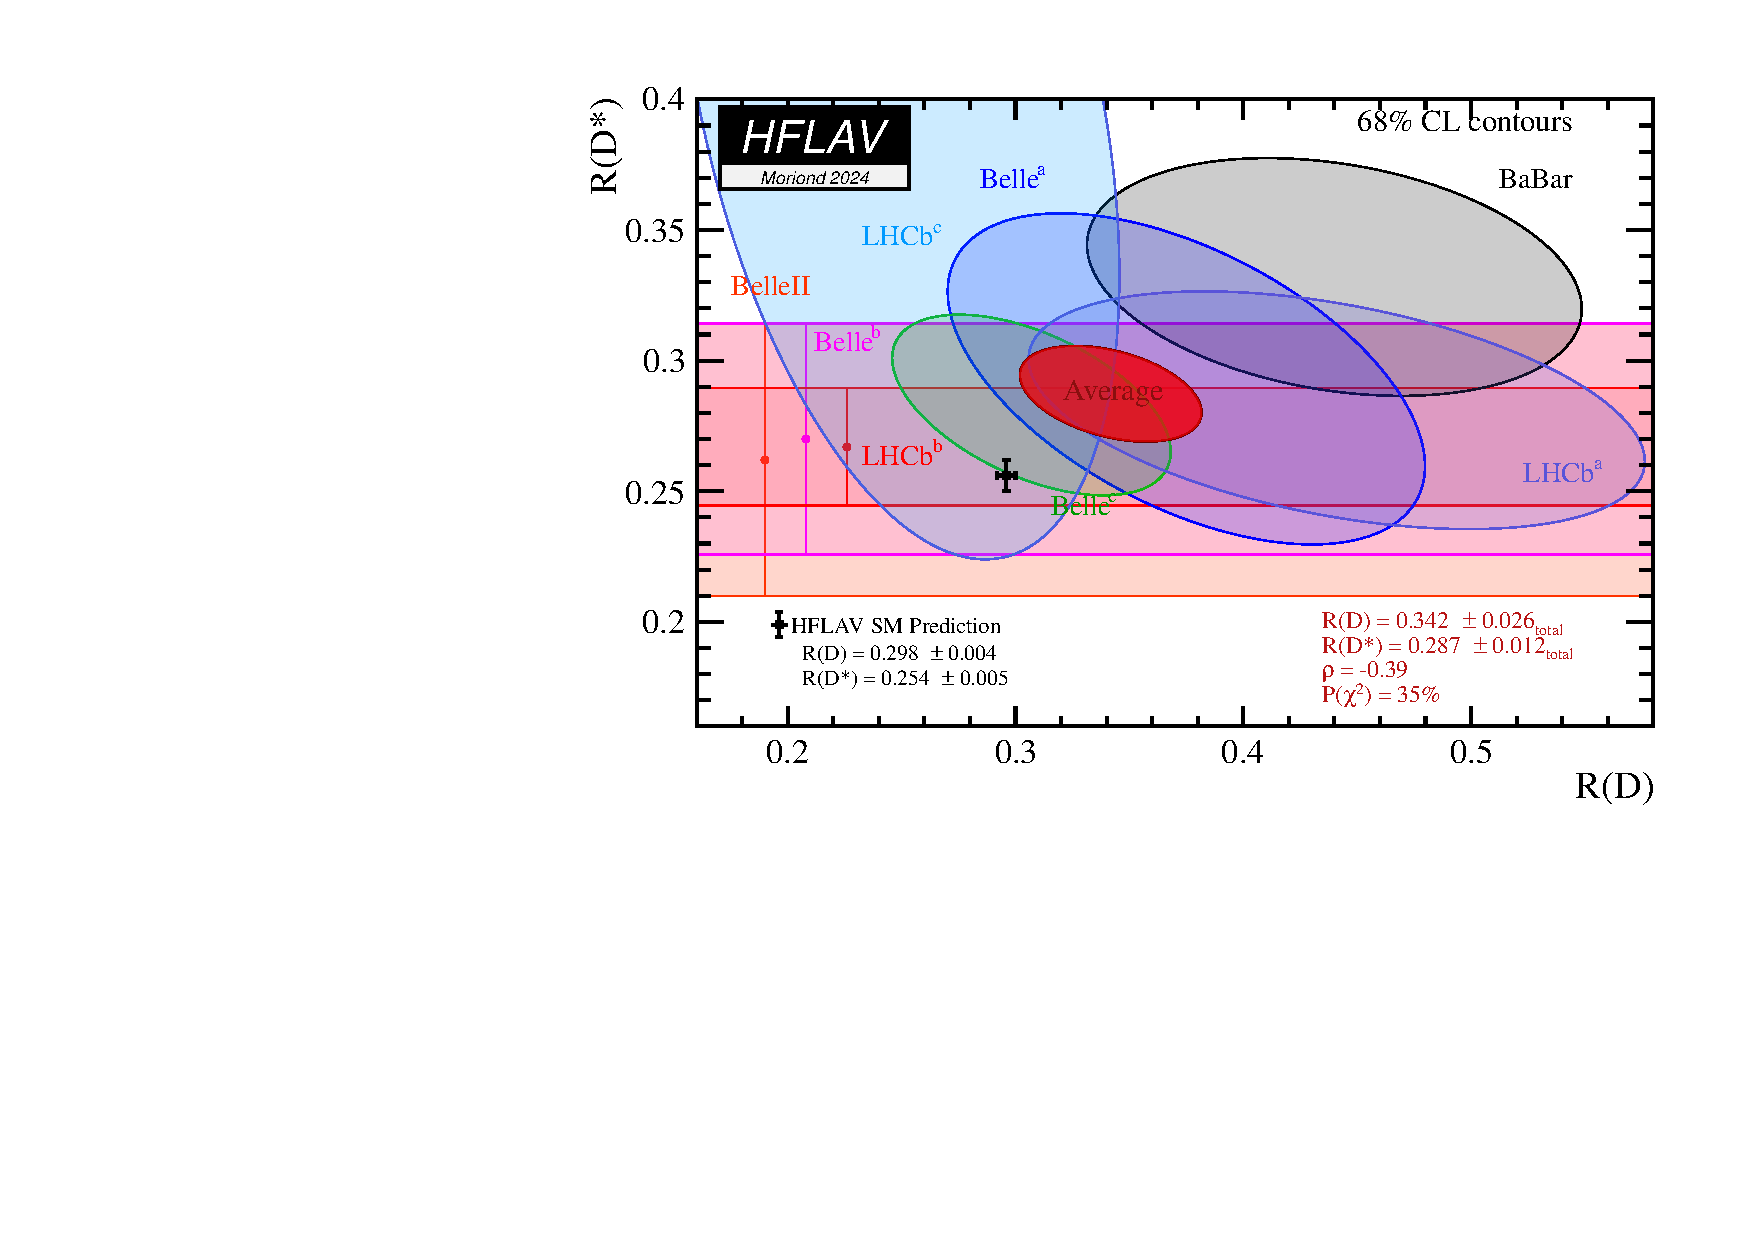
\includegraphics[width=.75\linewidth]{RDRDst_hflav.pdf}
	\end{center}
	\begin{equation}
		R(D)=\frac{\operatorname{BR}\left(B \rightarrow D \tau \nu\right)}{\operatorname{BR}\left(B \rightarrow D \ell_{(e,\mu)} \nu\right)},
		\quad
		R(D^{(*)})=\frac{\operatorname{BR}\left(B \rightarrow D^{(*)} \tau \nu\right)}{\operatorname{BR}\left(B \rightarrow D^{(*)} \ell_{(e,\mu)} \nu\right)}
	\end{equation}
\end{frame}


\begin{frame}{Leptoquarks and $R(D)$/ $R(D^*)$ anomalies}
	\begin{multicols}{2}
		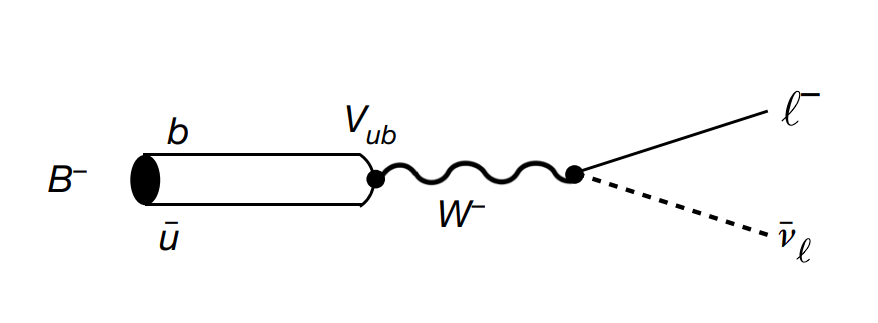
\includegraphics[width=.99\linewidth]{B_SM_1.png}
		$$ $$
		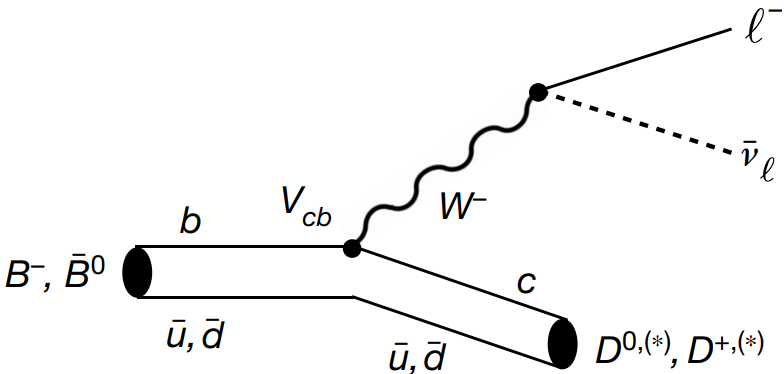
\includegraphics[width=.99\linewidth]{B_SM_2.png}
		\pause
		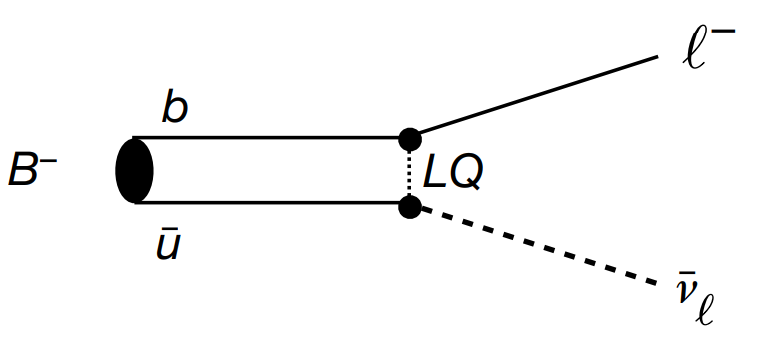
\includegraphics[width=.99\linewidth]{B_LQ_1.png}
		$$ $$
		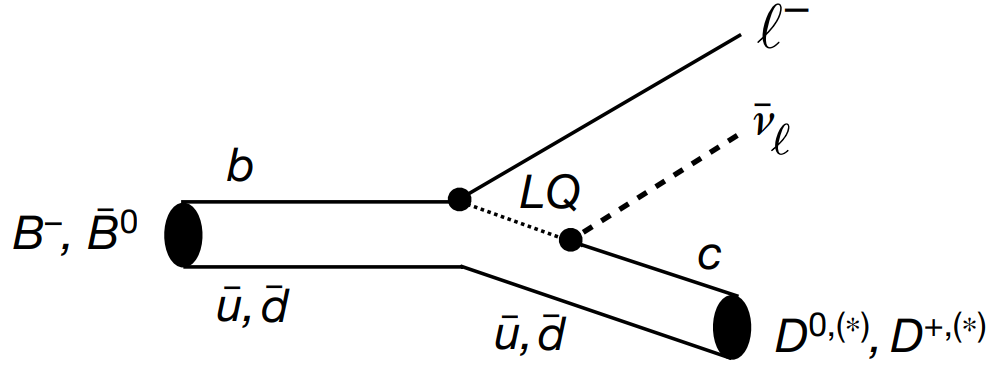
\includegraphics[width=.99\linewidth]{B_LQ_2.png}
	\end{multicols}
	\pause
	\begin{center}
		{\large $ $\\
		How can we test this hypothesis?
		}
	\end{center}
\end{frame}


\begin{frame}{Large Hadron Collider}{How can we test the leptoquark hypothesis?}
	\begin{minipage}{.55\linewidth}
		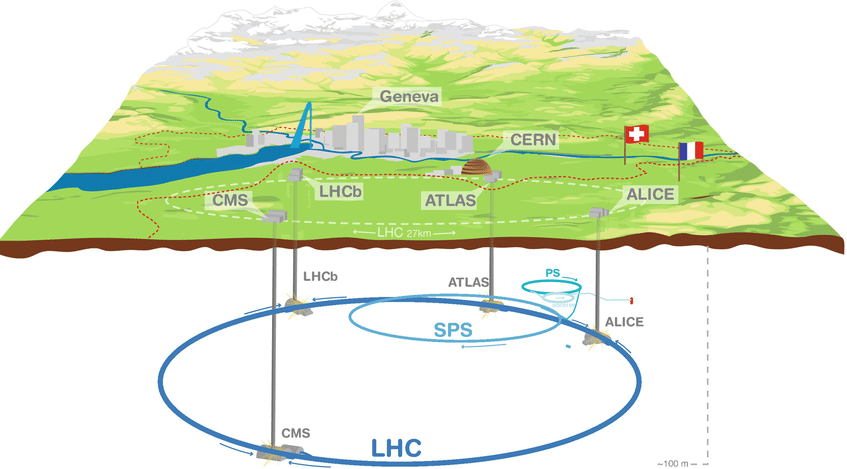
\includegraphics[width=.99\linewidth]{LHC.png}
	\end{minipage}
	\begin{minipage}{.42\linewidth}
		\begin{itemize}
			\item A Feasibility Study is needed.
			$$ $$
			\item Take Care on the dependence on the different parameters.
			$$ $$
			\item Take care on the content of particles.
			$$ $$
			\item Take care of the signal composition.$$ $$
			\item Take care on interference effects.
		\end{itemize}
	\end{minipage}
\end{frame}

% \begin{frame}{Large Hadron Collider}{How can we test the leptoquark hypothesis?}
% 	\begin{center}
% 		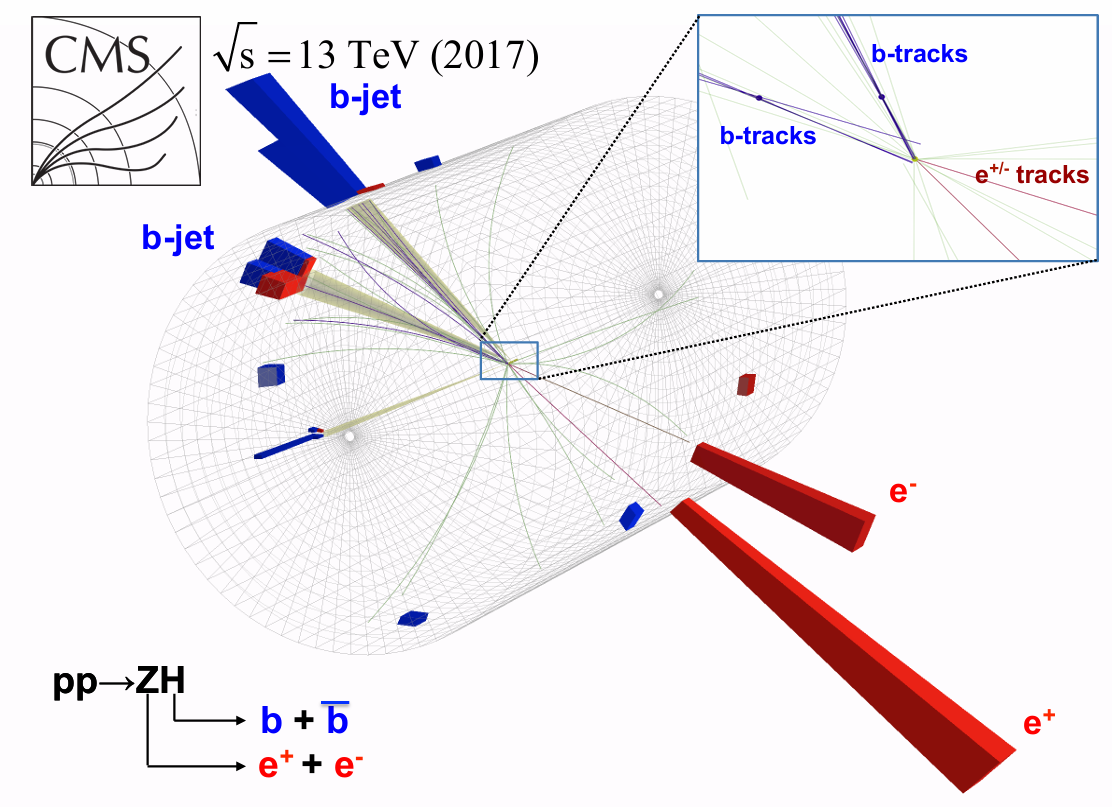
\includegraphics[width=.90\linewidth]{Collision.png}	
% 	\end{center}
% \end{frame}


\begin{frame}{Montecarlo Generators}
	

	\begin{center}
		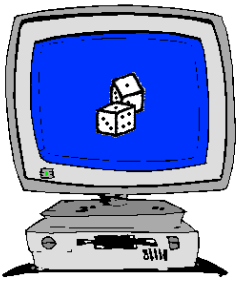
\includegraphics[scale=0.5]{A1}
	\end{center}

	Useful to predict what we expect to see under certain conditions:
	\begin{itemize}
		\item To perform studies before having the data
		\item To compute event selection efficiency/acceptance
		\item  To predict the ammount and composition of background events
		\item To distinguish different signals. 
	\end{itemize}
	
\end{frame}

\begin{frame}{Feasibility Studies Workflow}
	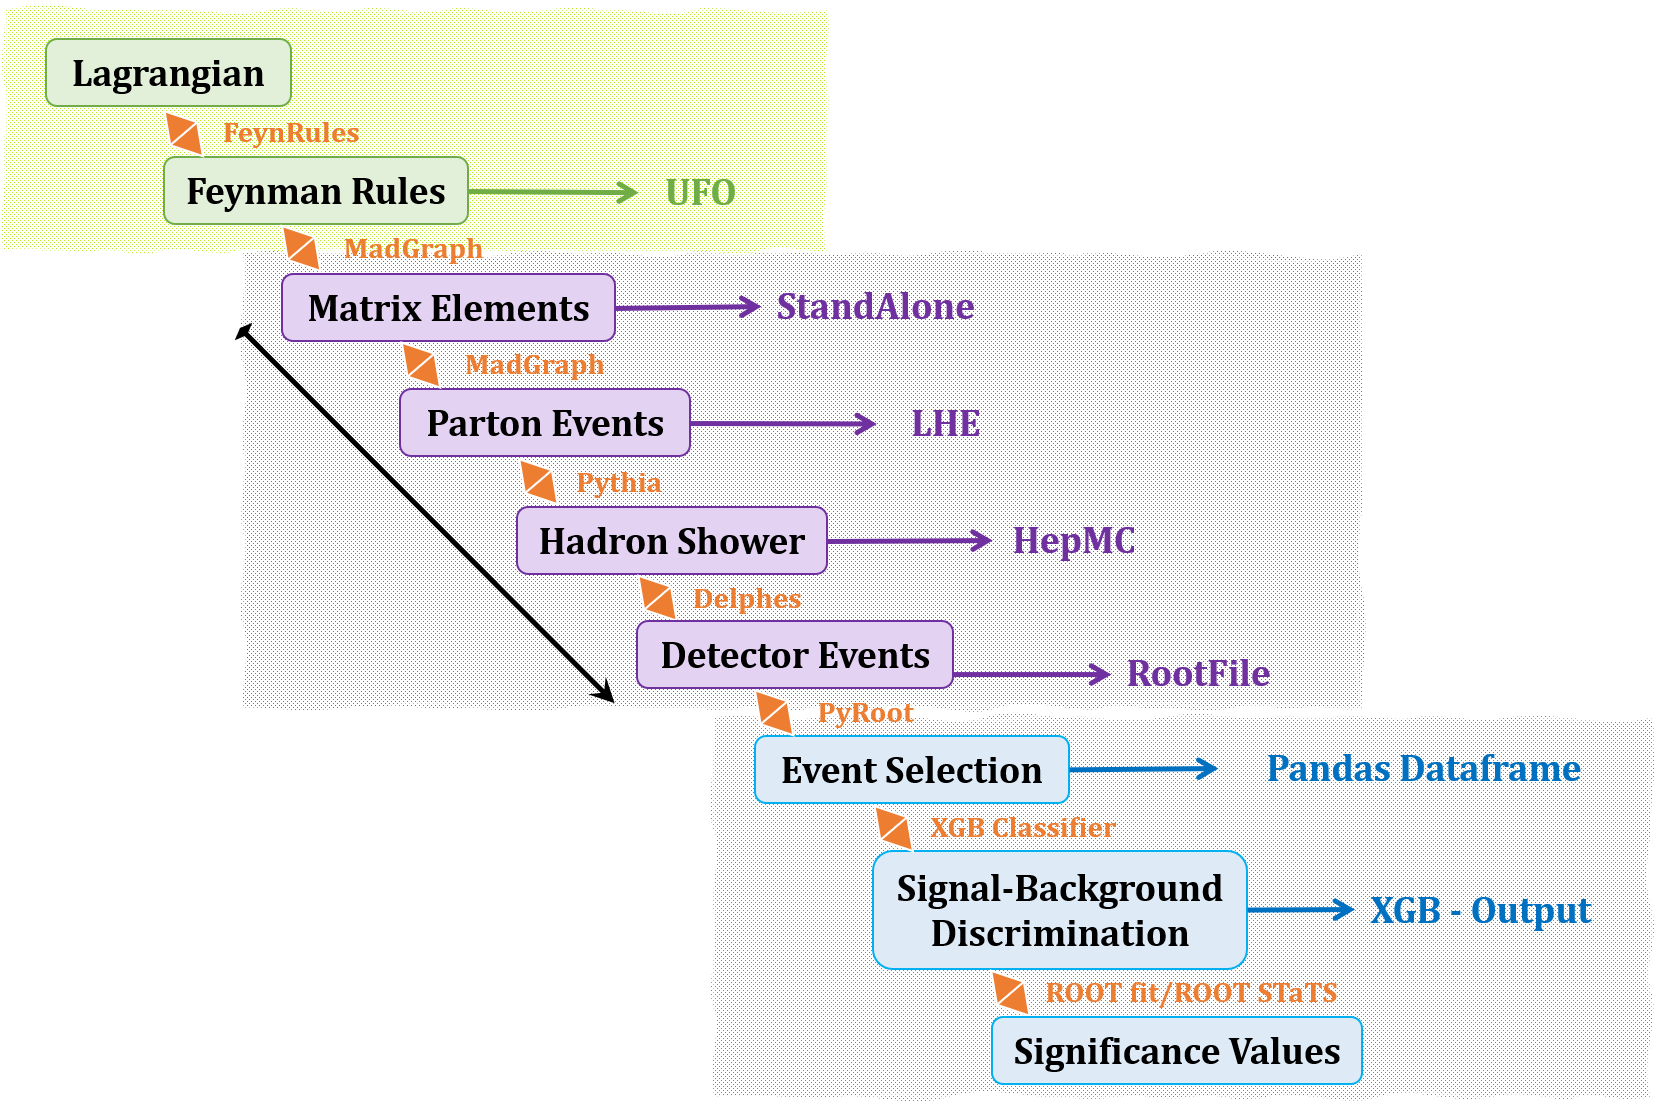
\includegraphics[width=1.0\linewidth]{Workflow.png}
\end{frame}

\begin{frame}{Vectorial Leptoquark Vertex}
	\begin{multicols}{2}
	A leptoquark is defined as a particle with a vertex that mix vectors and quarks.
	\begin{center}
	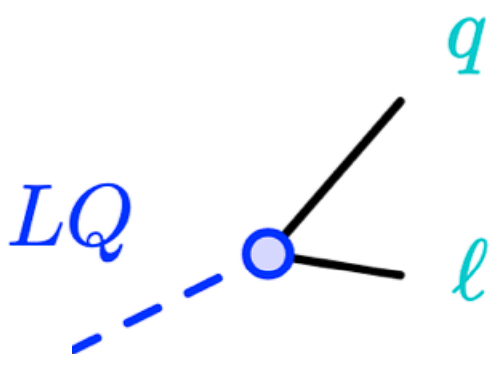
\includegraphics[width=.25\textwidth]{LQ_vertex.png}
	\end{center}
	If $U_1$ is a vector leptoquark that preserves the chirality on the vertex, we expect an interaction term like
	$$
	\sim U_1^\mu\bar{q}_{L} \gamma_{\mu} \ell_{L},
	$$
	and these allows a similar interaction term for the right handed currents 
	$$
	\sim U_1^\mu\bar{d}_{R} \gamma_{\mu} e_{R}.
	$$

	\end{multicols}
	Where the SM charges for the leptoquark, in the $Y=2(Q-T_3)$ convention, are
	\begin{center}
		\begin{tabular}{|c|c|c|c|c|}
			\hline & $\bar{q}_{L}$ & $\ell_{L}^{j}$ & $\bar{q}_{L}\gamma_{\mu} \ell_{L}$ & $U_{1}^{\mu}$ \\
			\hline$U(1)$ & $-1 / 3$ & $-1 $ & $-4 / 3$ & $+4 / 3$ \\
			\hline $\mathrm{SU}(2)$ & $\overline{\mathbf 2}$ & $\mathbf{2}$ & $\mathbf{1}$ & $\mathbf{1}$ \\
			\hline $\mathrm{SU}(3)$ & $\overline{\mathbf 3}$ & $\mathbf{1}$ & $\overline{\mathbf3}$ & $\mathbf{3}$ \\
			\hline
		\end{tabular}	
	\end{center}
	Then, the leptoquark $U_1 \sim \left(\mathbf{3}_{C}, \mathbf{1}_{I}, 4 / 3_{Y}\right)$, and its covariant derivative is
	$$
	\mathcal{D}_\mu U_\nu = \left(\partial_\mu+i g_s T^a G_\mu^a+ i \frac{2}{3} g' B_\mu \right)U_\nu.
	$$
\end{frame}

\begin{frame}{The Vector Leptoquark Lagrangian}
	
	The full Lagrangian for the vector leptoquark is
	\begin{align*}
		\mathcal{L}_{U}=&-\frac{1}{2} U_{\mu \nu}^{\dagger} U^{\mu \nu}+M_{U}^{2} U_{\mu}^{\dagger} U^{\mu}\\&-i g_{s}\left(1-\kappa_{c}\right) U_{\mu}^{\dagger} T^{a} U_{\nu} G^{\mu \nu}_a -\frac{2 i}{3} g'\left(1-\kappa_{Y}\right) U_{\mu}^{\dagger} U_{\nu} B^{\mu \nu}\\
		&+\frac{g_{U}}{\sqrt{2}}\left[U_{1}^{\mu}\left(\beta_{L}^{i j} \bar{q}_{L}^{i} \gamma_{\mu} e_{L}^{j}+\beta_{R}^{i j} \bar{d}_{R}^{i} \gamma_{\mu} e_{R}^{j}
		%+\beta_{N}^{i} \bar{u}_{R}^{i} \gamma_{\mu} N_{R}
		\right)+\text { h.c. }\right]
	\end{align*}
	where $U_{\mu \nu}=\mathcal D_{\mu} U_{\nu}-\mathcal D_{\nu} U_{\mu}$, $\mathcal D_{\mu}=\partial_{\mu}-i g_{s} G_{\mu}^{a} T^{a}-i \frac{2}{3} g_{Y} B_{\mu}$, and the couplings $\beta_{L}$ and $\beta_{R}$ are complex $3 \times 3$ matrices in flavor space. If $U_1$ has a gauge origin $\kappa_{c}=\kappa_{Y}=0$.
	\pause
	Defining 
	$$
	\psi_{L}^{\mathrm{SM}}=\begin{pmatrix}
		q_{Lr}\\ q_{Lg}\\ q_{Lb}\\ \ell_L
	\end{pmatrix}
	\Longrightarrow\;\;
	\mathcal{L}_{\text{int}}
	\sim U_{1\alpha}^\mu \bar{\psi}_{L}^{\mathrm{SM}}\, \gamma_{\mu} T_{+}^{\alpha } \psi_{L}^{\mathrm{SM}} + \text{h.c.},
	\quad
	T_{+}^{\alpha}=\begin{pmatrix}
		0 & 0 & 0 & \delta_{r\alpha}\\
		0 & 0 & 0 & \delta_{g\alpha}\\
		0 & 0 & 0 & \delta_{b\alpha}\\
		0 & 0 & 0 & 0
	\end{pmatrix},
	$$
	we have six generators $T_{\pm}^{\alpha }$ with closure relation,
	$$
	\sum_{\alpha} \left[{T_{+}^{\alpha }},{T_{-}^{\alpha}}\right] =
	3 T_{B-L}=\begin{pmatrix}
		1 & 0 & 0 & 0\\
		0 & 1 & 0 & 0\\
		0 & 0 & 1 & 0\\
		0 & 0 & 0 & -3
	\end{pmatrix}.
	$$
	So, the gauge group with this leptoquark must include a $U(1)_{B-L}$ symmetry. The right-handed currents also have a similar interaction term.
\end{frame}

\begin{frame}{Take care, you could need a $Z'$ boson}
	The generator $T_{B-L}$ is associated with the $U(1)_{B-L}$ symmetry with a $Z'$ boson. The interaction terms for the $Z'$ boson have the form
	\begin{align*}
		\mathcal{L}_{\text{int}} &\sim Z'_\mu\left(\bar{\psi}_{L}^{\mathrm{SM}}\gamma^\mu (3T_{B-L}) \psi_{L}^{\mathrm{SM}}\right)\\
		&\sim Z'_\mu \left(\bar q_{L} \gamma^\mu q_{L} - 3 \bar \ell_L \gamma^\mu \ell_L\right).
	\end{align*}\pause
	so, the full Lagrangian for the $Z'$ boson is
	\begin{equation}
		\begin{aligned}
		\mathcal{L}_{Z^{\prime}}= & -\frac{1}{4} Z_{\mu \nu}^{\prime} Z^{\prime \mu \nu} +\frac{1}{2} M_{Z^{\prime}}^2 Z_\mu^{\prime} Z^{\prime \mu} \\
		& +\frac{g_{Z^{\prime}} }{2 \sqrt{6}} Z^{\prime \mu}\left(\zeta_q^{i j} \bar{q}_L^i \gamma_\mu q_L^j+\zeta_u^{i j} \bar{u}_R^i \gamma_\mu u_R^j+\zeta_d^{i j} \bar{d}_R^i \gamma_\mu d_R^j-3 \zeta_{\ell}^{i j} \bar{\ell}_L^i \gamma_\mu \ell_L^j-3 \zeta_e^{i j} \bar{e}_R^i \gamma_\mu e_R^j\right),
		\end{aligned}
	\end{equation}
	where the couplings $\zeta$ are complex $3\times 3$ matrices in flavor space.\pause

	\vfill
	We assume that both, the $Z'$ and the vector leptoquark $U_1$, have preferential couplings to third generation fermions, so $\beta^{33}\gg \beta^{ij}$ and $\zeta^{33}\gg \zeta^{ij}$.
\end{frame}

\begin{frame}{Feynrules}
	\begin{center}
		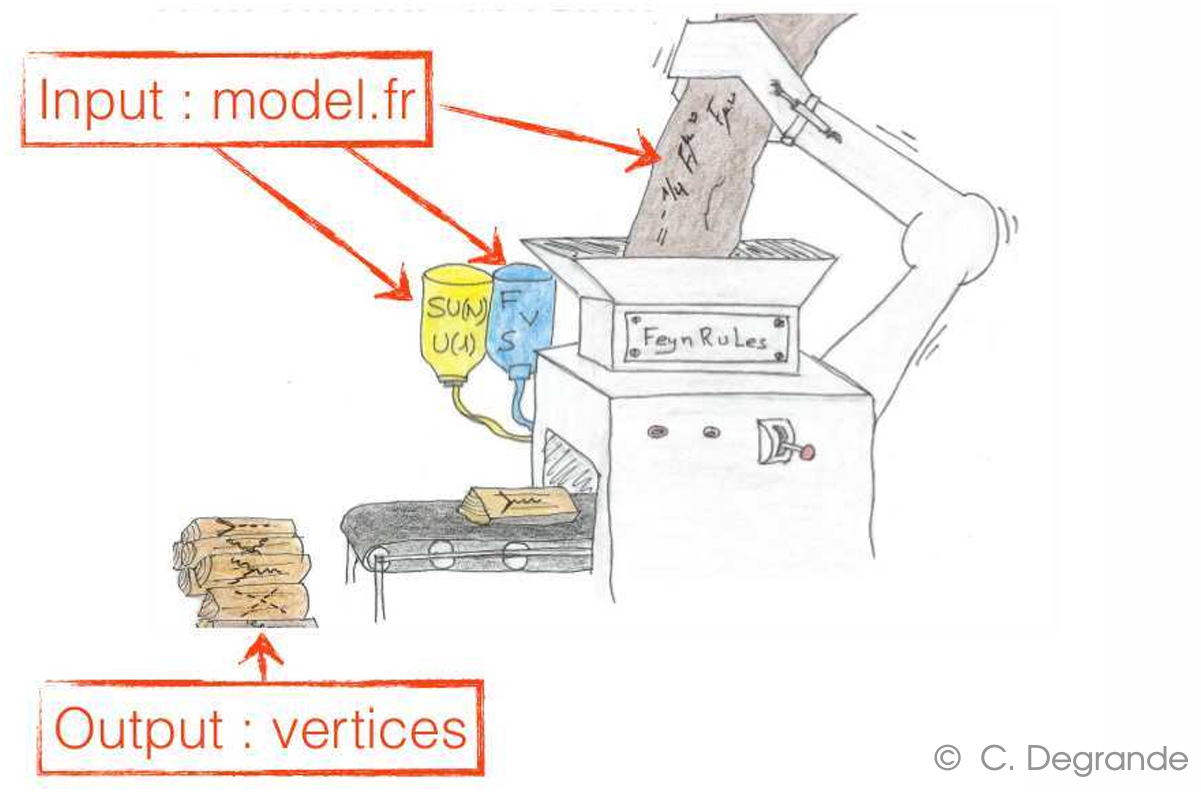
\includegraphics[width=.99\linewidth]{Feynrules.png}
	\end{center}
\end{frame}

\begin{frame}{Madgraph-Pythia8-Delphes for the LHC}
	\begin{center}
		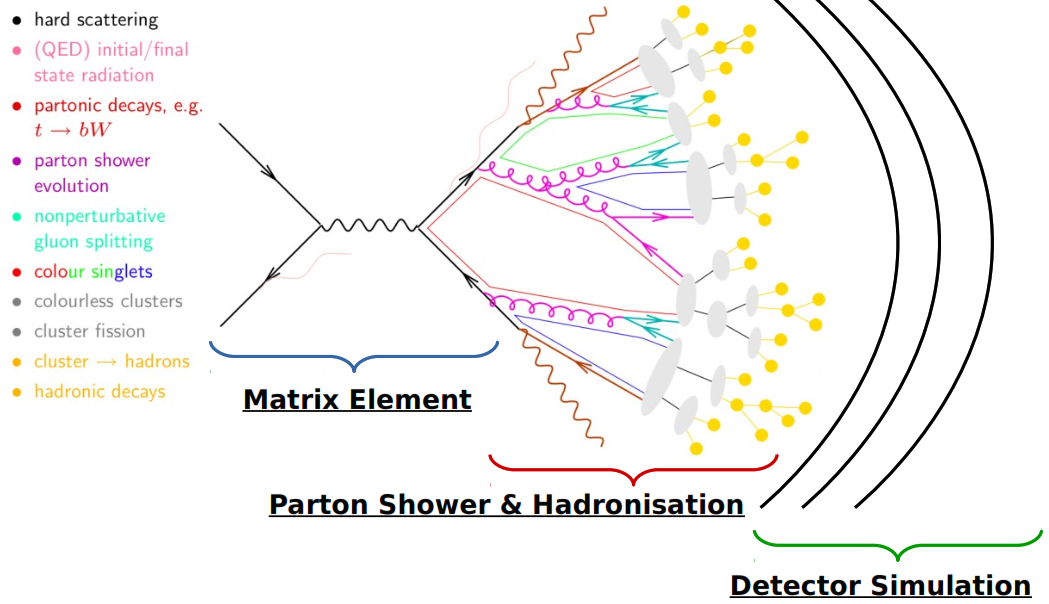
\includegraphics[width=.99\linewidth]{Madgraph.png}
	\end{center}
\end{frame}

\begin{frame}{Leptoquark Production at pp Colliders}
	\begin{center}
		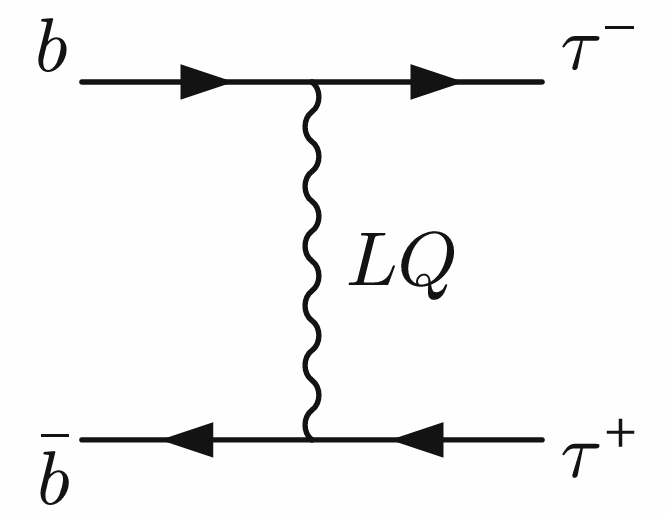
\includegraphics[width=.30\textwidth]{non_resonant.png}\hfill
		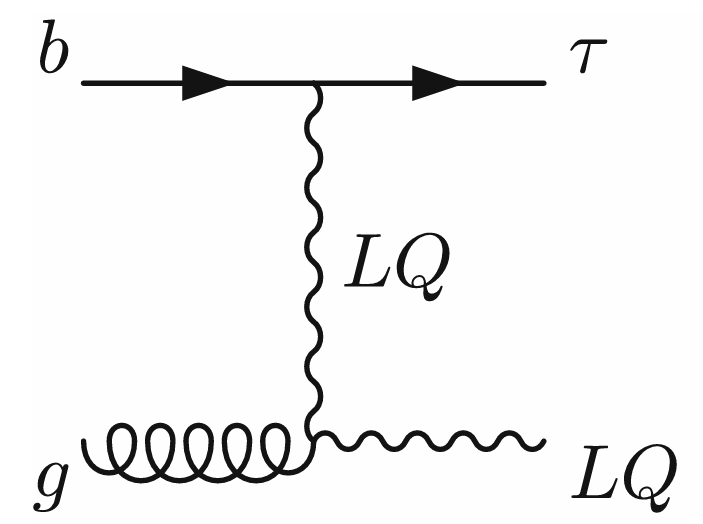
\includegraphics[width=.30\textwidth]{single_LQ.png}\hfill
		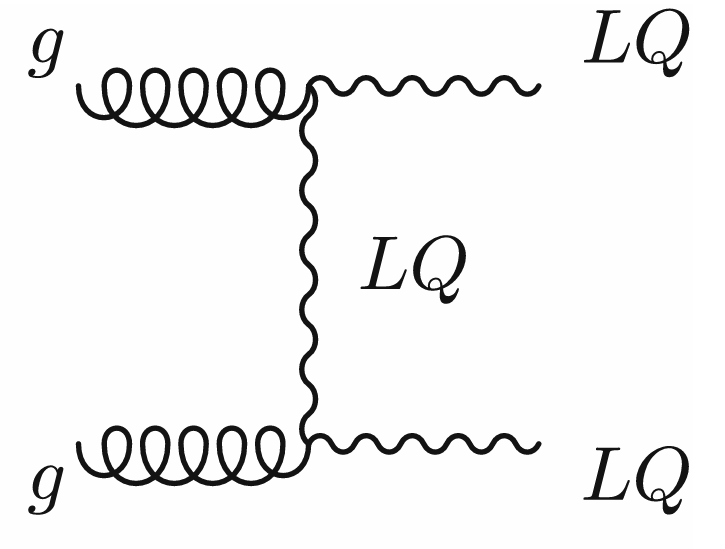
\includegraphics[width=.30\textwidth]{double_LQ.png}
	\end{center}\pause
	\begin{center}
		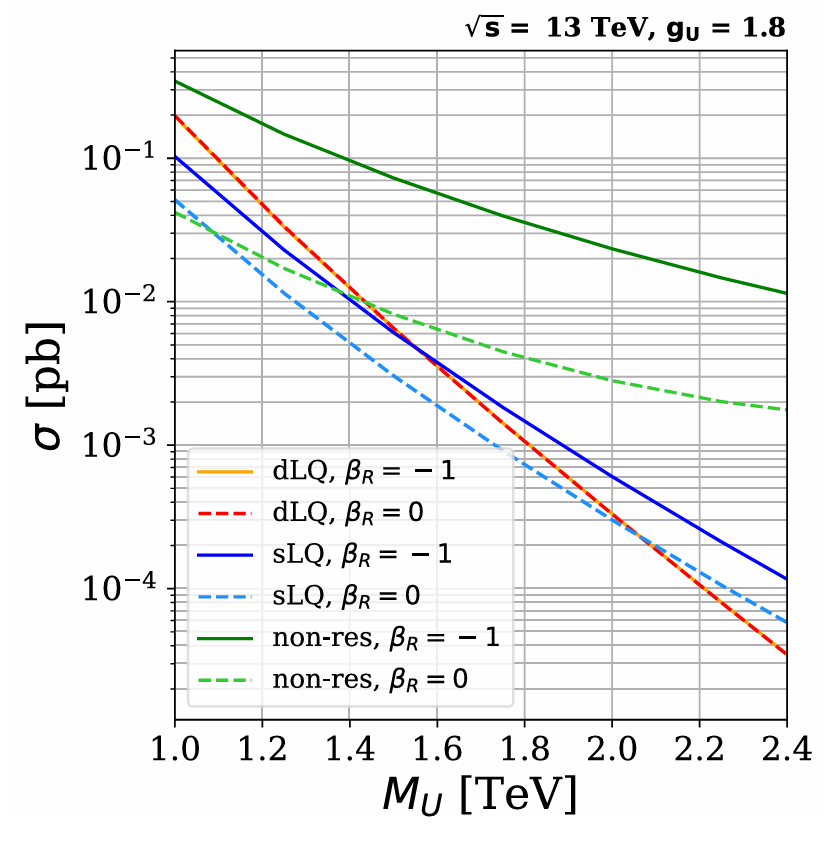
\includegraphics[width=.45\textwidth]{XS.png}
		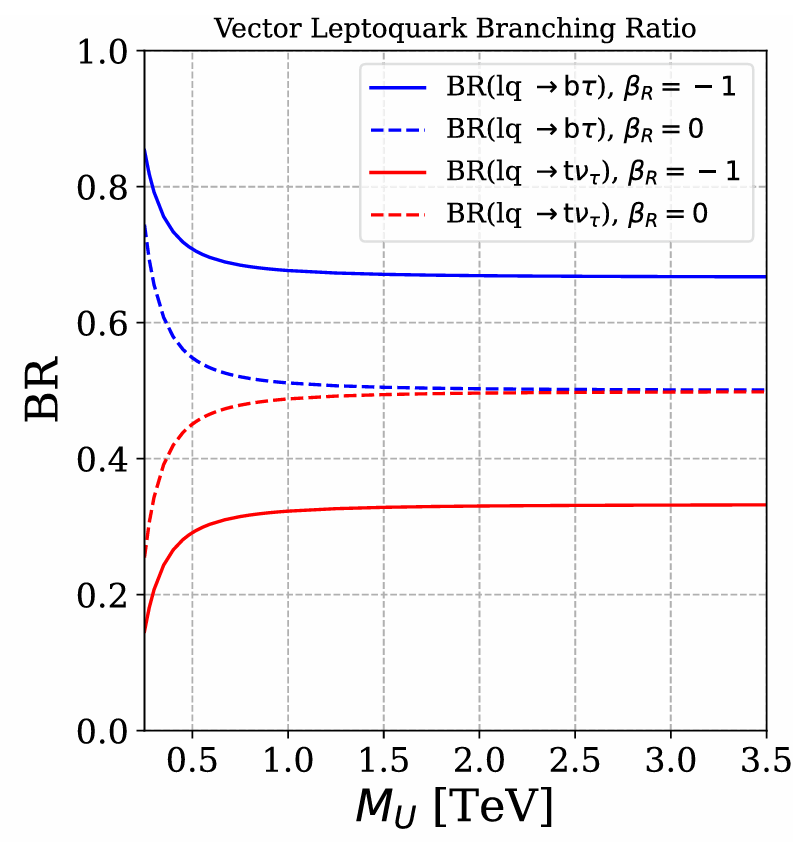
\includegraphics[width=.45\textwidth]{BR.png}
	\end{center}
\end{frame}

\begin{frame}{Interferences between the $Z'$ and the Vector Leptoquark}

	\begin{minipage}{.50\linewidth}
		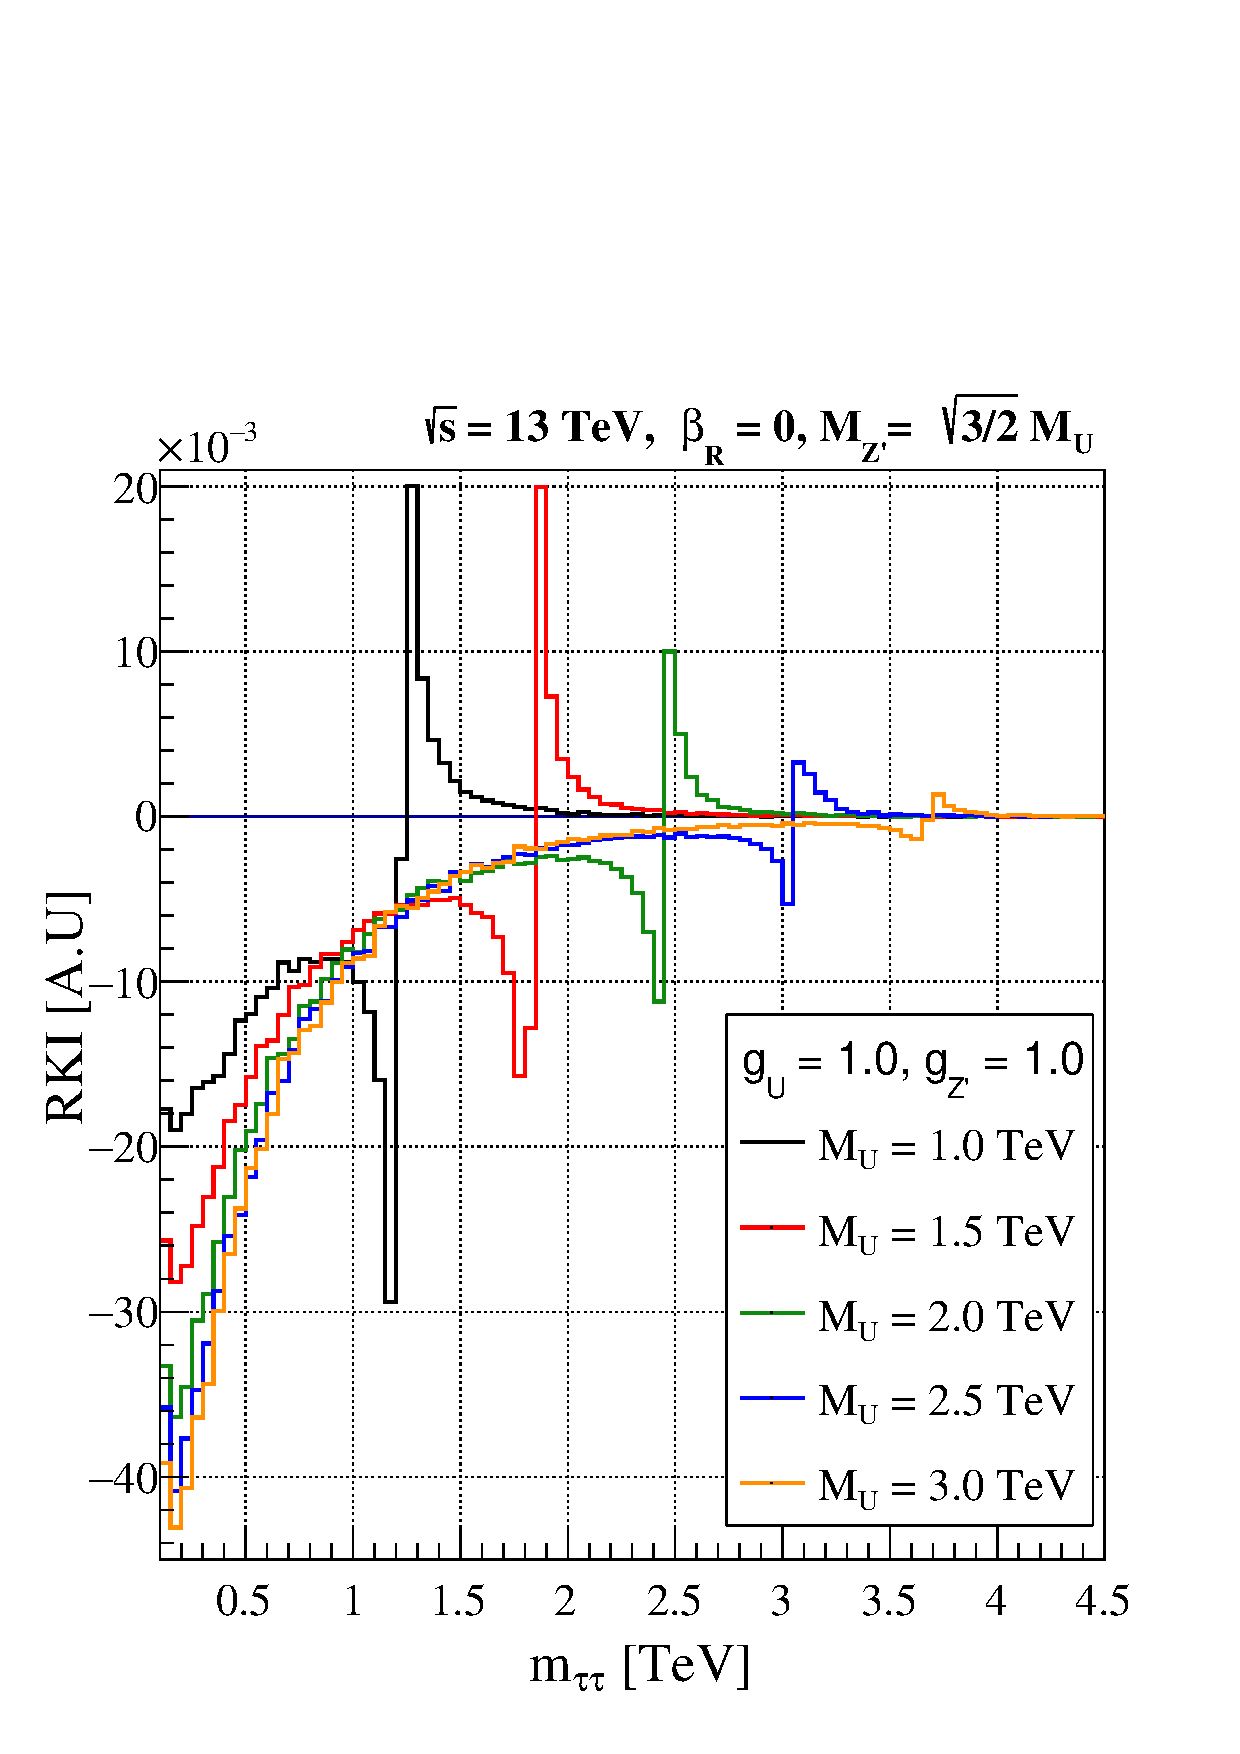
\includegraphics[width=\linewidth]{Kinematic_Interference_gu_1.0_gzp_1.0_zp_upper_limit_woRHC.pdf}
	\end{minipage}
	\begin{minipage}{.48\linewidth}
		\begin{center}
			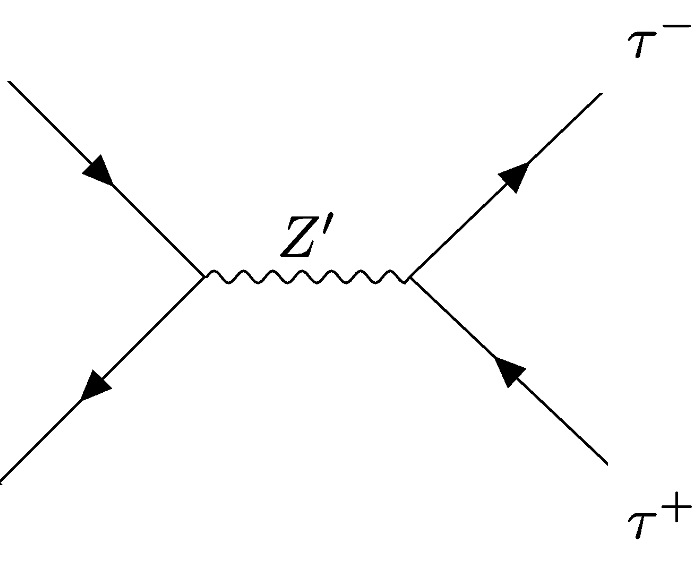
\includegraphics[width=\linewidth]{Zp.png}
		\end{center}

		\begin{equation*}
			\mathrm{RKI}=\frac{1}{\sigma_{ LQ+Z'}}\left[\frac{d\sigma_{ LQ+Z'}}{dm_{\tau\tau}}-\left(\frac{d\sigma_{ LQ}}{dm_{\tau\tau}}+\frac{d\sigma_{Z'}}{dm_{\tau\tau}}\right)\right]
		\end{equation*}
	\end{minipage}	
\end{frame}

\begin{frame}{Interferences between the $Z'$ and the Vector Leptoquark}
	\begin{center}
		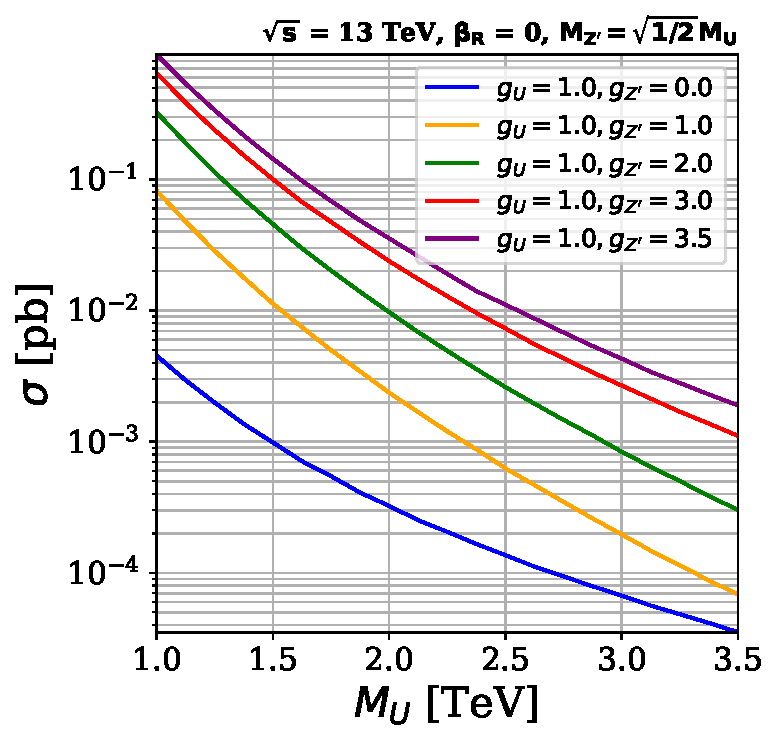
\includegraphics[width=.48\linewidth]{XS_gu_gzp_lower_limit_woRHC.pdf}
		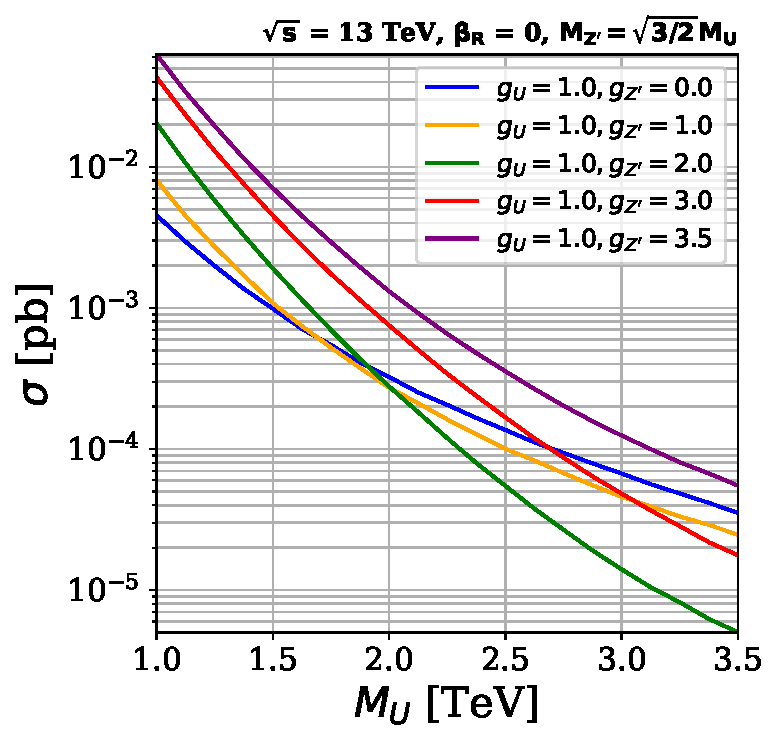
\includegraphics[width=.48\linewidth]{XS_gu_gzp_upper_limit_woRHC.pdf}
	\end{center}
	{\large 
		For large values of the couplings, the interference between the $Z'$ and the vector leptoquark mainly destructive, so the cross-section is reduced.
	}
\end{frame}

\begin{frame}{Tau Desintegration Modes}
	\begin{center}
		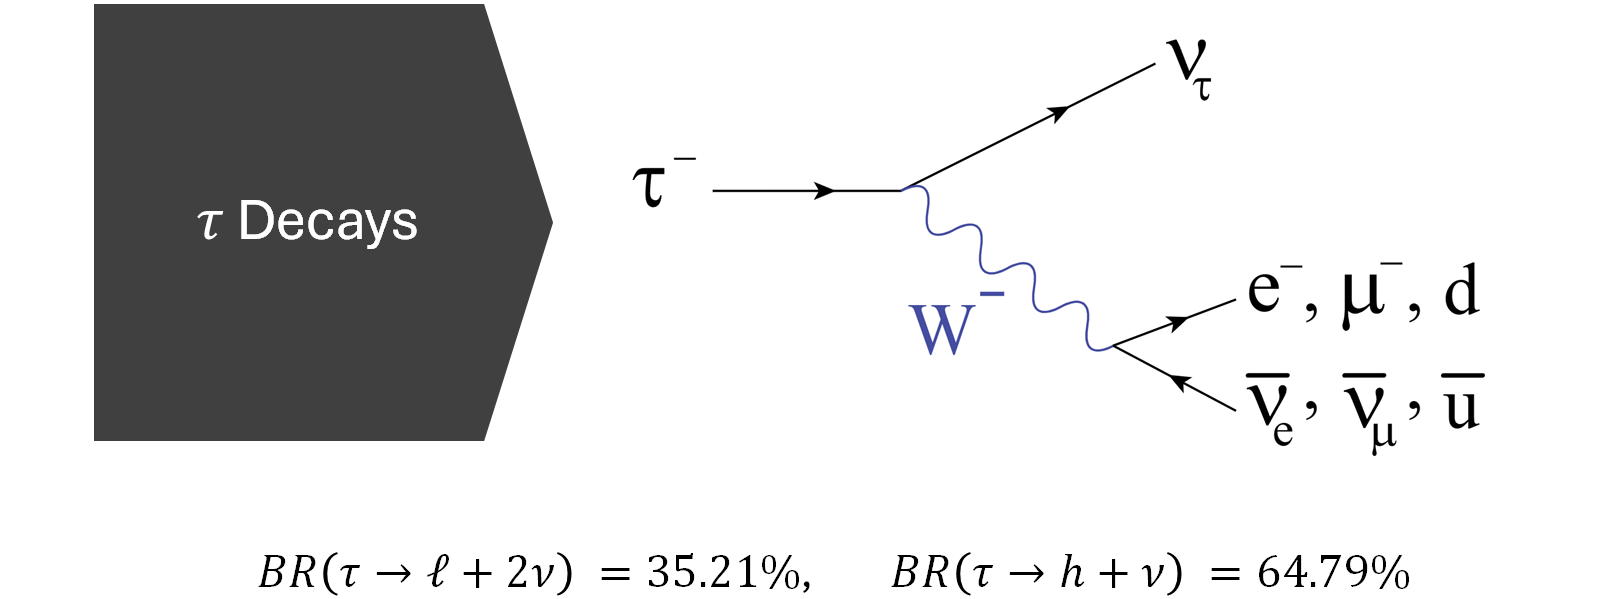
\includegraphics[width=.99\linewidth]{tau_decays.png}
		$$ $$\pause
		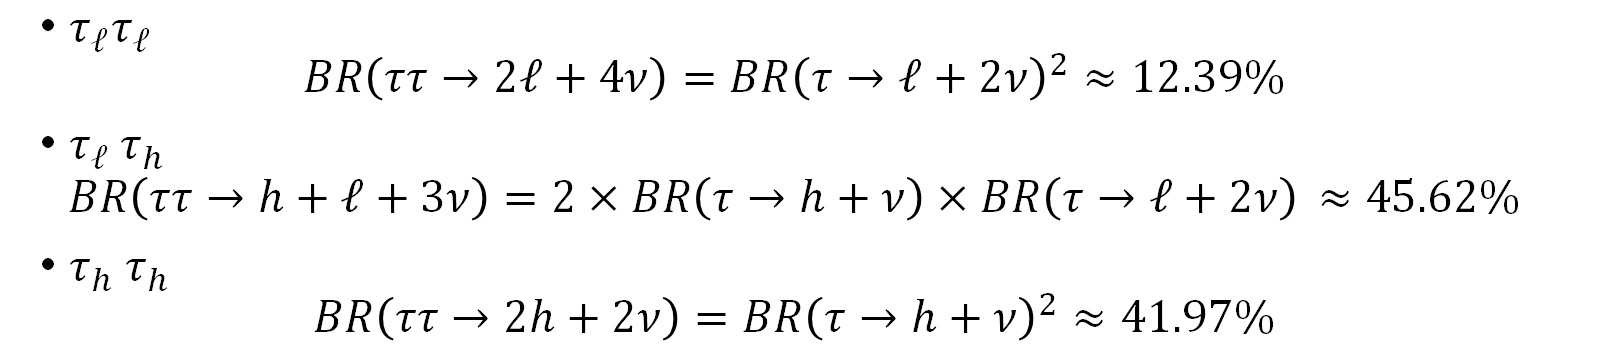
\includegraphics[width=.99\linewidth]{tau_decays2.png}
	\end{center}
\end{frame}

\begin{frame}{Kinematic Variables}
	\begin{center}
		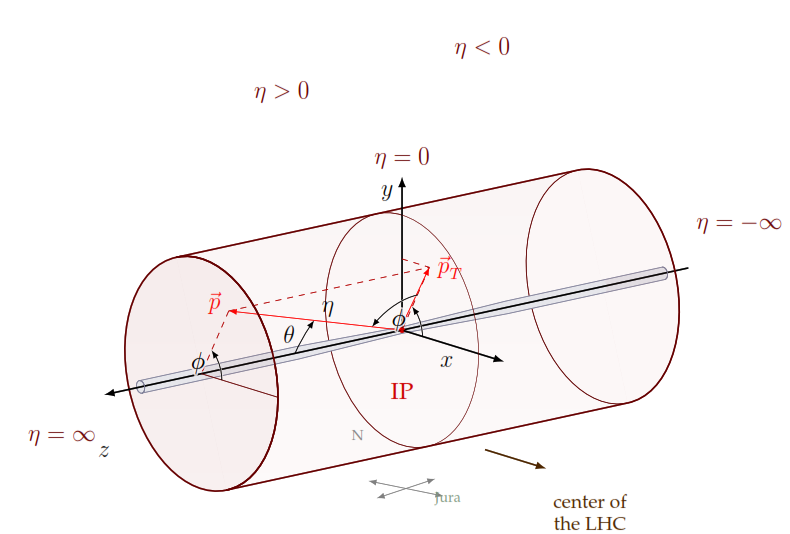
\includegraphics[width=.99\linewidth]{Kinematic_Variables.png}
	\end{center}
\end{frame}

\begin{frame}{Preselection Criteria}
	\begin{center}
		\large
		\begin{tabular}{|c|cccccc|}
\hline
\multirow{2}{*}{\textbf{Variable}} & \multicolumn{6}{c|}{\textbf{Threshold}} \bigstrut\\ 
\cline{2-7} 
                                   & \multicolumn{1}{c|}{$\tau_{h} \tau_{h}$} & \multicolumn{1}{c|}{$b \tau_{h} \tau_{h}$} & \multicolumn{1}{c|}{$b b \tau_{h} \tau_{h}$} & \multicolumn{1}{c|}{$\tau_{h} \tau_{\ell}$} & \multicolumn{1}{c|}{$b \tau_{h} \tau_{\ell}$} & $b b \tau_{h} \tau_{\ell}$ \bigstrut\\ \hline \hline


$N(b)$                             & \multicolumn{1}{c|}{= 0} & \multicolumn{1}{c|}{= 1} & \multicolumn{1}{c|}{$\geq 2$} & \multicolumn{1}{c|}{= 0}& \multicolumn{1}{c|}{= 1} & $\geq 2$ \bigstrut\\ \hline
$p_T(b)$                         & \multicolumn{1}{c|}{-} & \multicolumn{2}{c|}{$\geq 30 \textrm{GeV}$ } & \multicolumn{1}{c|}{-} & \multicolumn{2}{c|}{$\geq 30 \textrm{GeV}$ } \bigstrut\\ \hline
$|\eta(b)|$                        & \multicolumn{1}{c|}{-} &\multicolumn{2}{c|}{$\leq 2.4$} & \multicolumn{1}{c|}{-} &\multicolumn{2}{c|}{$\leq 2.4$} \bigstrut\\ \hline
                                  
$N (\ell)$                         & \multicolumn{3}{c|}{= 0}  & \multicolumn{3}{c|}{= 1} \bigstrut\\ \hline
$N(\tau_{h})$                      & \multicolumn{3}{c|}{ $= 2$} & \multicolumn{3}{c|}{= 1} \bigstrut\\ \hline
$p_T(\ell)$                         & \multicolumn{3}{c|}{-} & \multicolumn{3}{c|}{$\geq 35 \textrm{GeV}$} \bigstrut\\ \hline
$p_T(\mu)$                       & \multicolumn{3}{c|}{-} & \multicolumn{3}{c|}{$\geq 30 \textrm{GeV}$} \bigstrut\\ \hline
$|\eta(\ell)|$                     & \multicolumn{3}{c|}{-} & \multicolumn{3}{c|}{$\leq 2.4$} \bigstrut\\ \hline
$p_T(\tau_h)$                    & \multicolumn{6}{c|}{$\geq 50$ GeV} \bigstrut\\ \hline
$|\eta(\tau_h)|$                   & \multicolumn{6}{c|}{$\leq 2.3$} \bigstrut\\ \hline
$\Delta R(p_{i}, p_{j})$           & \multicolumn{6}{c|}{$\geq 0.3$} \bigstrut\\ \hline

\end{tabular}

	\end{center}
\end{frame}

\begin{frame}{$S_T^{\text{meT}}=\text{met} + \sum_i\left|p_{T}^i\right|$}
	\begin{center}
		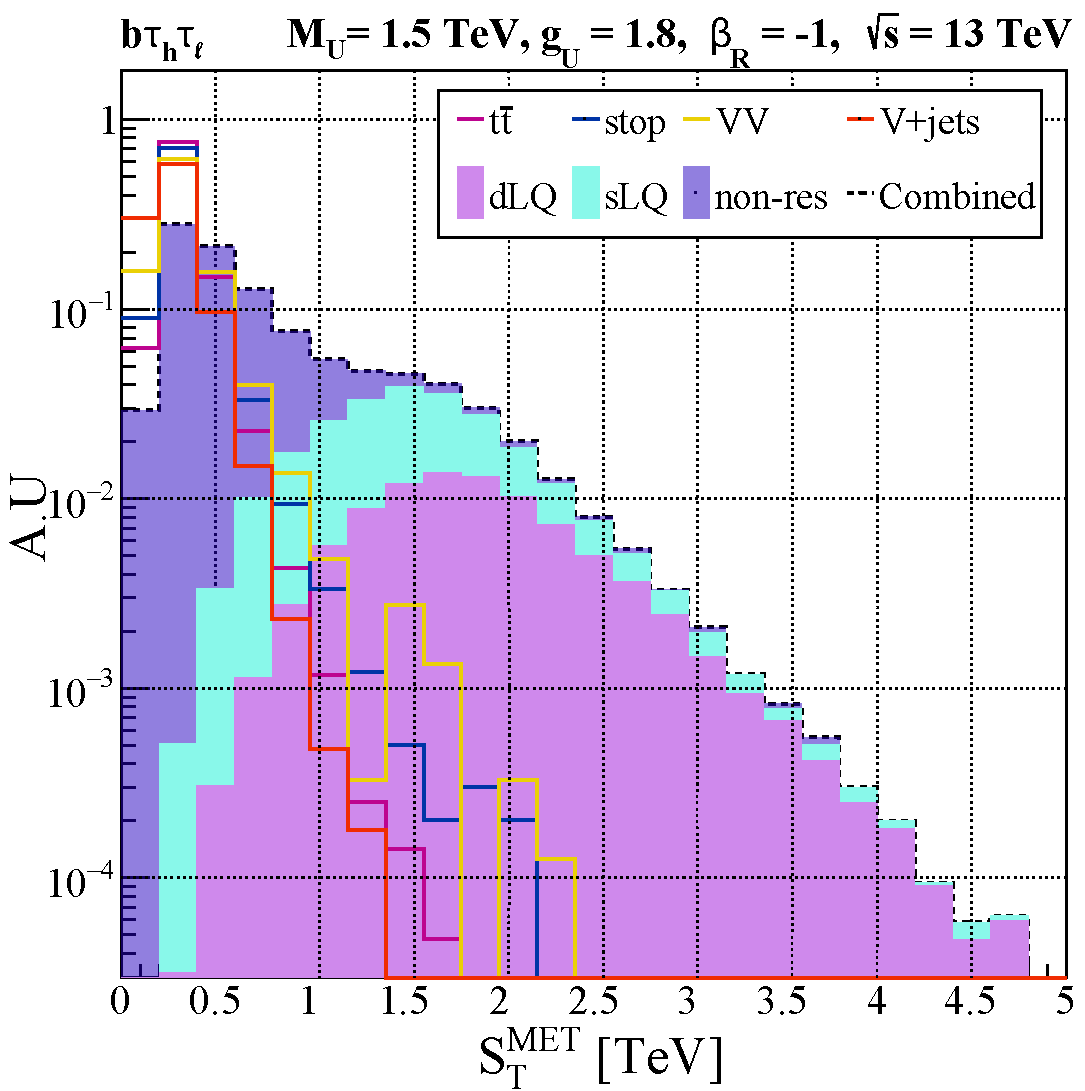
\includegraphics[width=.65\linewidth]{sTTeV_semileptonic_sLQ_wRHC.pdf}
	\end{center}
	
\end{frame}

\begin{frame}{$\Delta R = \sqrt{\Delta \eta^2 + \Delta \phi^2}$}
	\begin{center}
		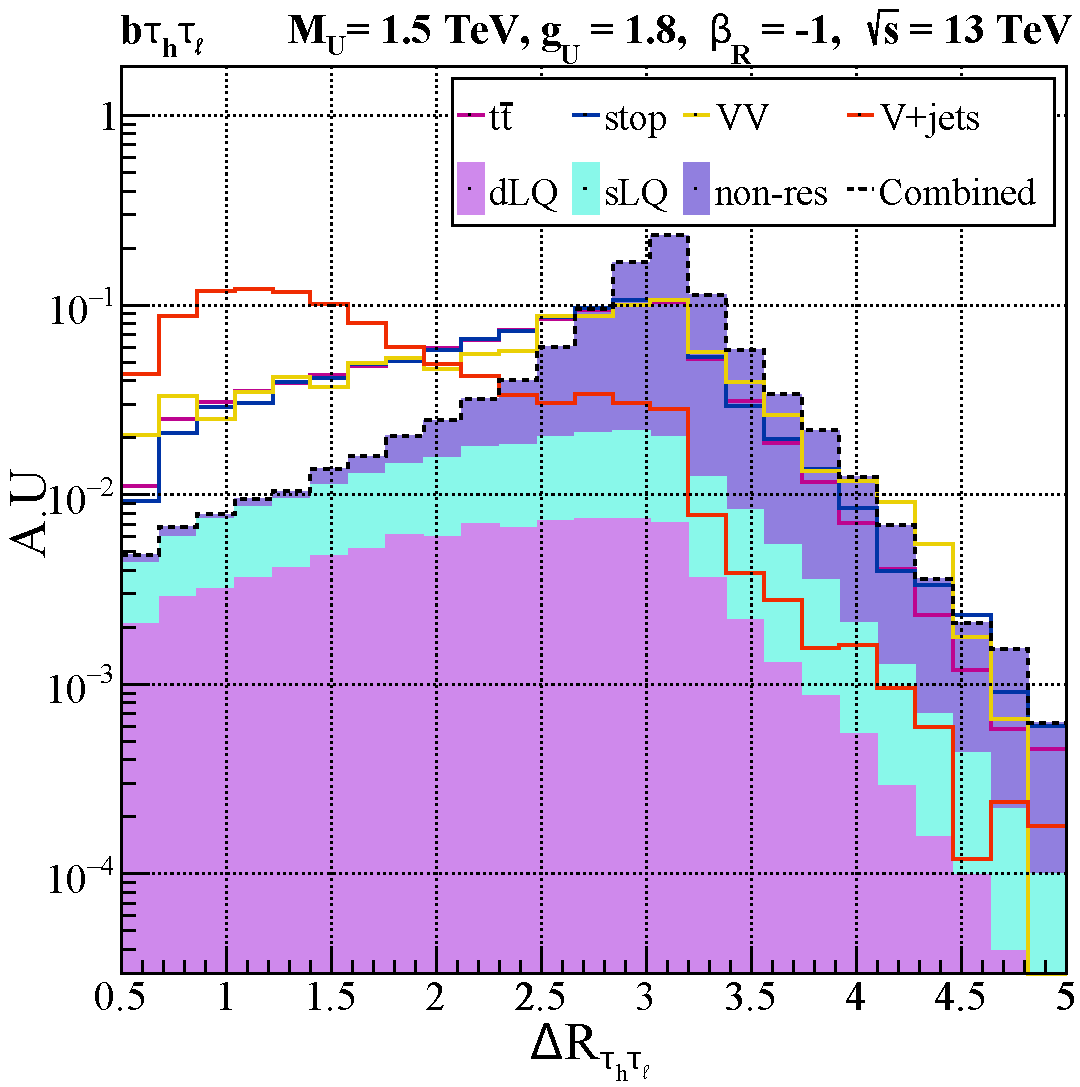
\includegraphics[width=.65\linewidth]{DeltaR_semileptonic_sLQ_wRHC.pdf}	
	\end{center}
	
\end{frame}


\begin{frame}{Boosted Decision Tree}
	\begin{center}
		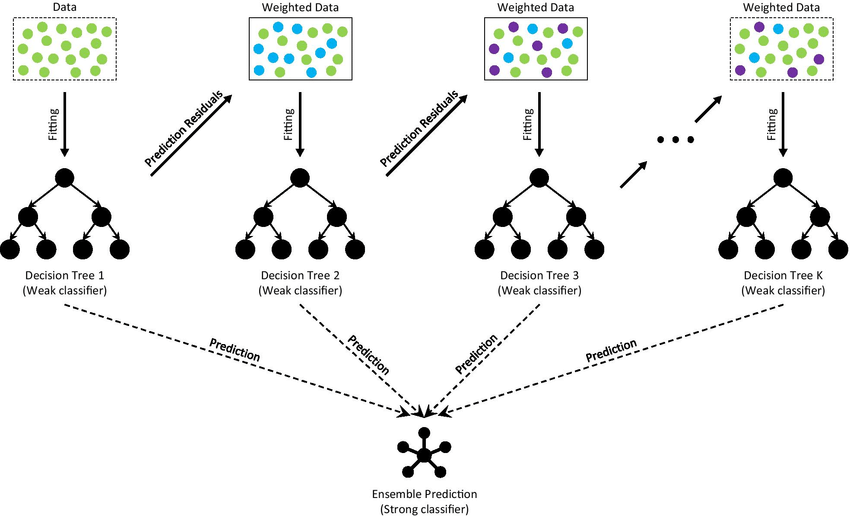
\includegraphics[width=1.0\linewidth]{BDT.png}
	\end{center}
\end{frame}


\begin{frame}{Cross-Validation}
	\begin{center}
		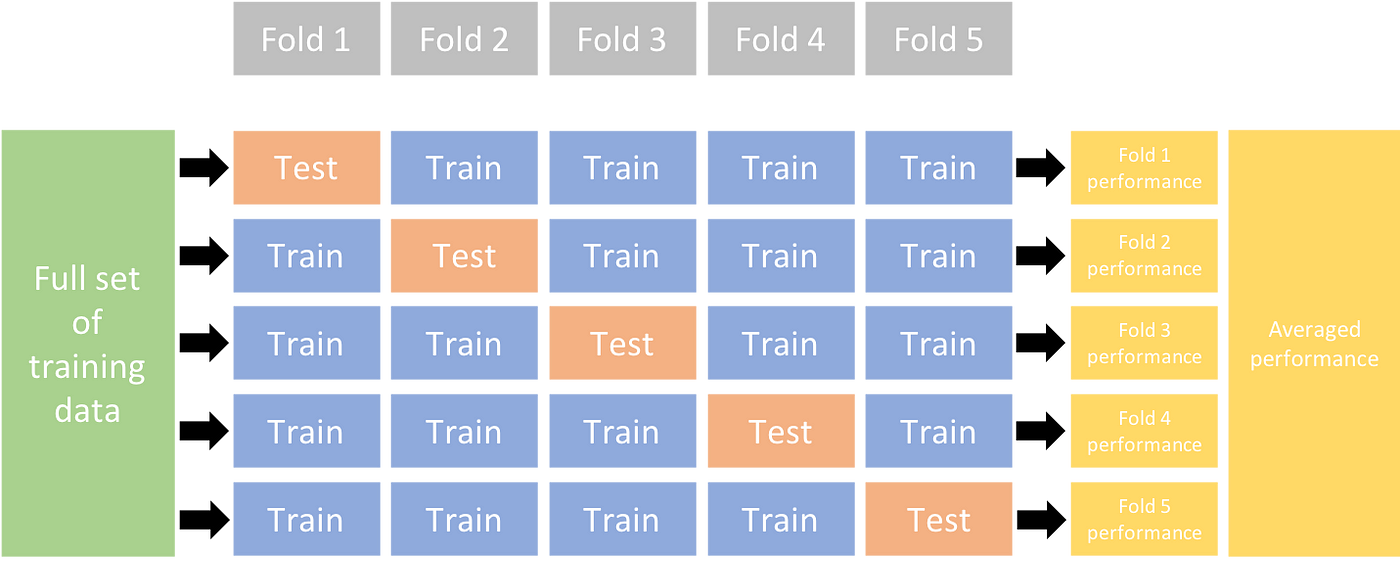
\includegraphics[width=1.0\linewidth]{CV.png}
	\end{center}

	We made this for the XGBoost discriminator algorithm with a 10-fold cross-validation for each point in the hyperparameter space:
	\begin{itemize}
		\item \texttt{max\_depth} $\in \{3, 5, 7, 9\}$
		\item \texttt{learning\_rate} $\in \{ 0.01, 0.1, 1, 10\}$
		\item \texttt{n\_estimators} $\in \{75, 125, 250, 500\}$
	\end{itemize}
	So, we have one optimized discriminator for each mass point, each channel, and each value of $\beta_R^{33}$.

\end{frame}

\begin{frame}{The optimized observable}{XGB-output}

	We can evaluate a score for the signal and background events using the discriminator algorithm. 

	\begin{center}
		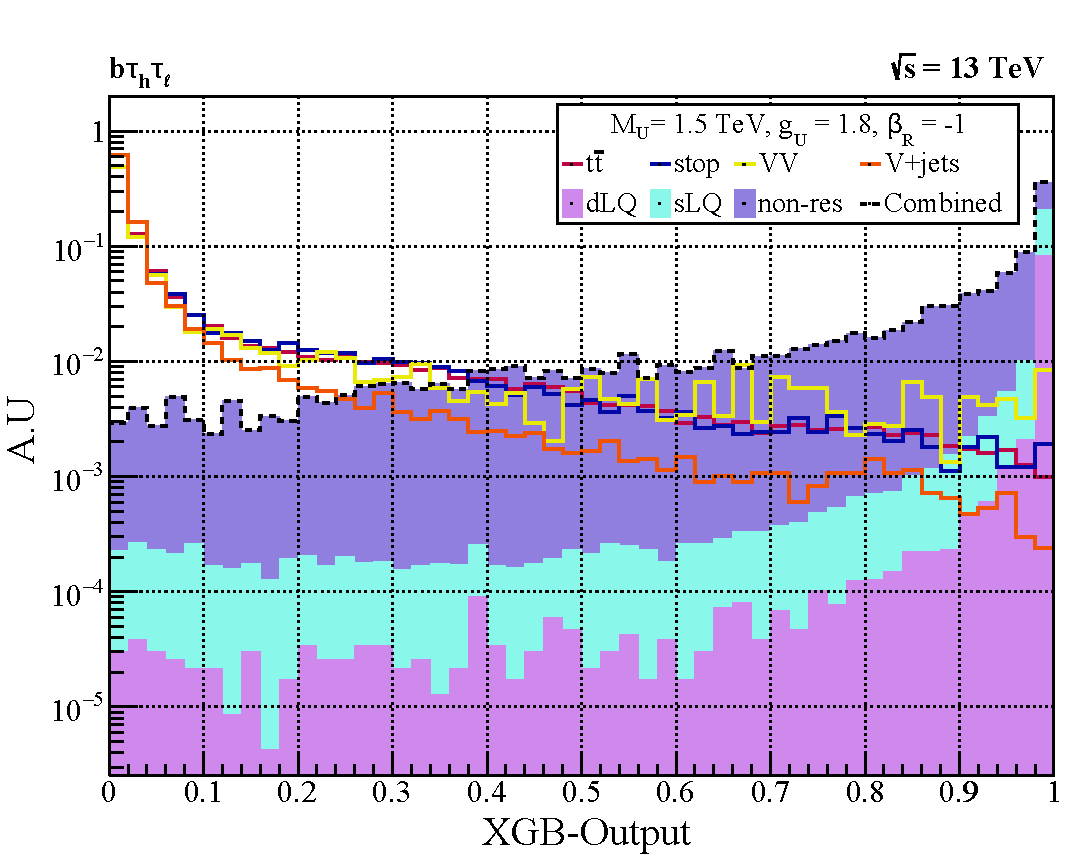
\includegraphics[width=.75\linewidth]{ML_semileptonic_sLQ_wRHC.pdf}
	\end{center}
		
\end{frame}

\begin{frame}{Hunting Peaks and Tails}{Searches for New Physics}
	\begin{multicols}{2}
		One can construct a test that estimates how significant the deviation from the background in a distribution:
		$$
		k'=\frac{N^{(hyp)}-N^{(null)}}{\sigma_{N^{(hyp)}}}.
		$$
		\vfill
		If $S$ and $B$ are the number of events for the signal and background, then
		$$
		k'=\frac{S}{\sqrt{S+B}}.
		$$

		\begin{center}
			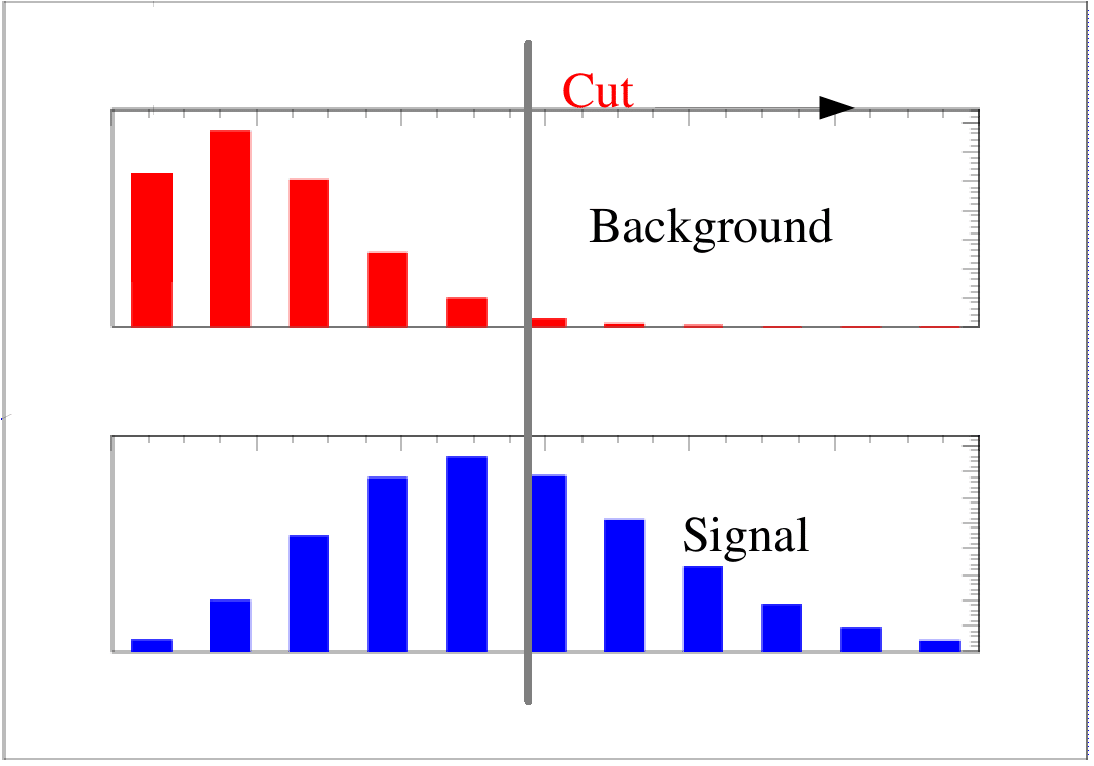
\includegraphics[width=.75\linewidth]{simpleopt-06.png}
		\end{center}
		\pause 
		If you add gaussian systematic uncertainties, then
		$$
		k'=\frac{S}{\sqrt{S+B+\delta_{\text{sys}}^2}}.
		$$

		\pause

		If we treat each bin as an independent Poisson variable and we add the systematic uncertainties, then
		$$
		\boxed{
			k \approx \frac{\sum_i w_i S_i}{\sqrt{\sum_i w_i^2 (S_i+B_i+\delta_{\text{sys}}^2)}},
		}
		$$
		where $w_i = A \ln \left(1+\frac{S_i}{B_i}\right)$, with $A$ a normalization constant, is the weight for each bin.
	\end{multicols}

\end{frame}

\begin{frame}{Double Leptoquark Production}{The Sensitivity Reach / only left-handed currents}
	\begin{minipage}{.30\linewidth}
		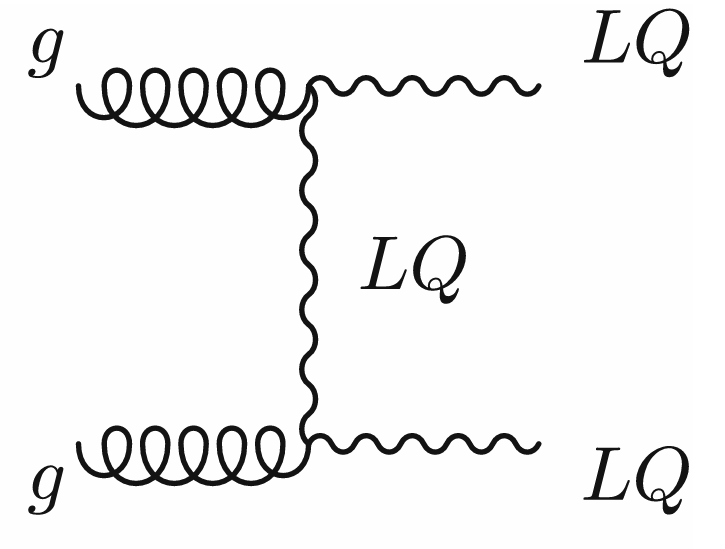
\includegraphics[width=\linewidth]{double_LQ.png}
	\end{minipage}
	\begin{minipage}{.68\linewidth}
		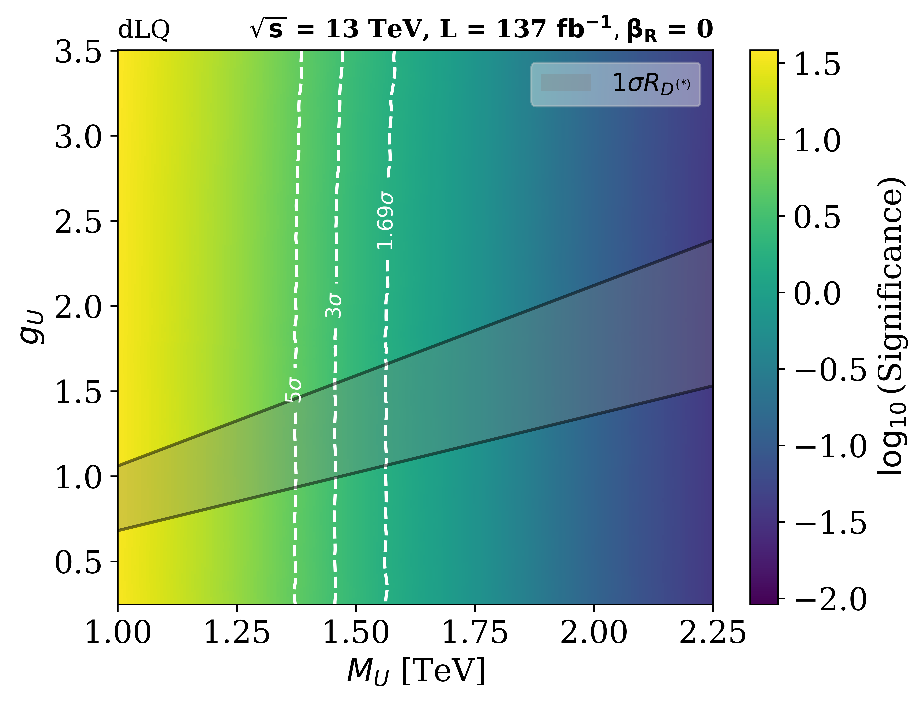
\includegraphics[width=\linewidth]{Significance_Heatmap_13TeV_L137_dLQ_combined_woRHC.pdf}
	\end{minipage}
	{\large
	  Double leptoquark production is sensitive to the leptoquark mass, its production depends only on the QCD coupling constant and the available energy.
	}
\end{frame}

\begin{frame}{Single leptoquark production}{The Sensitivity Reach / only left-handed currents}
	\begin{minipage}{.30\linewidth}
		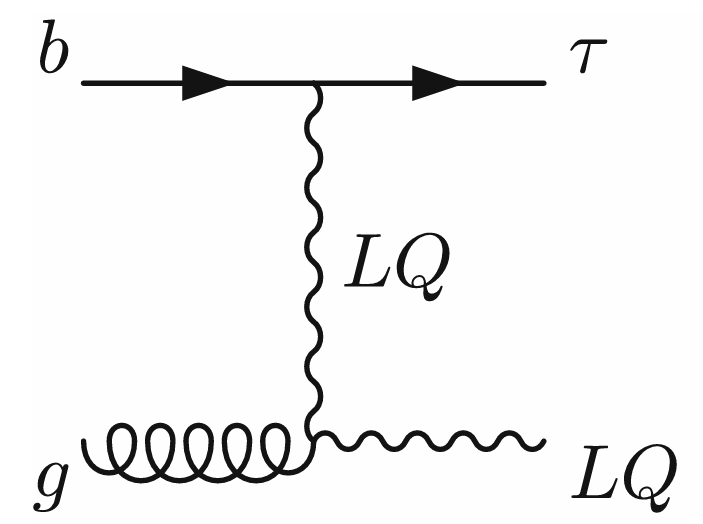
\includegraphics[width=\linewidth]{single_LQ.png}
	\end{minipage}
	\begin{minipage}{.68\linewidth}
		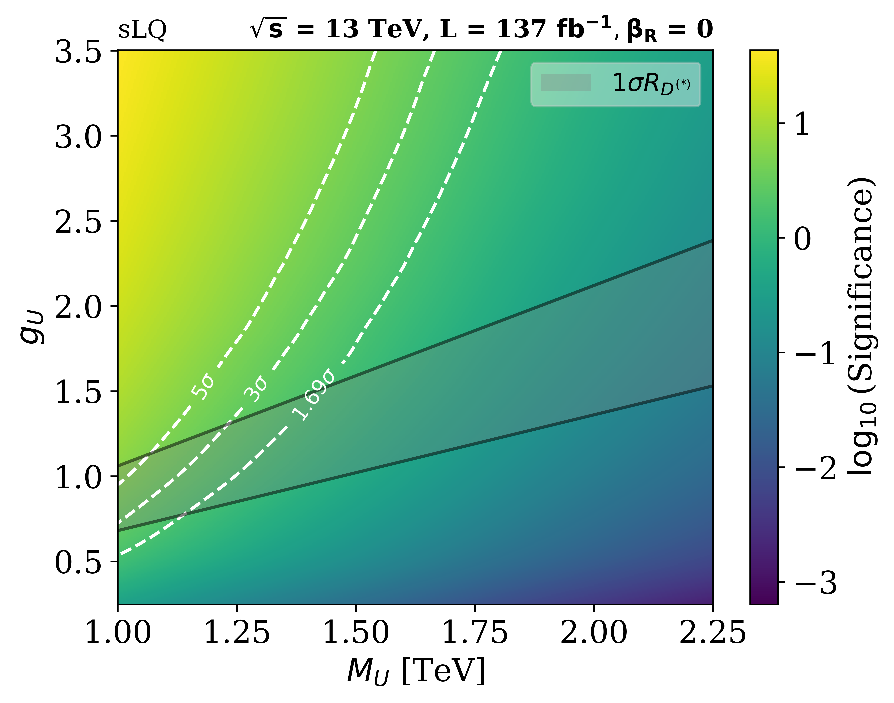
\includegraphics[width=\linewidth]{Significance_Heatmap_13TeV_L137_sLQ_combined_woRHC.pdf}
	\end{minipage}
	{\large
		  Single leptoquark production is sensitive to both, mass and couplings. It contributes to the regions of high coupling constants at higher masses than double leptoquark production.
	}
\end{frame}

\begin{frame}{Non-resonant Production}{The Sensitivity Reach / only left-handed currents}
	\begin{minipage}{.30\linewidth}
		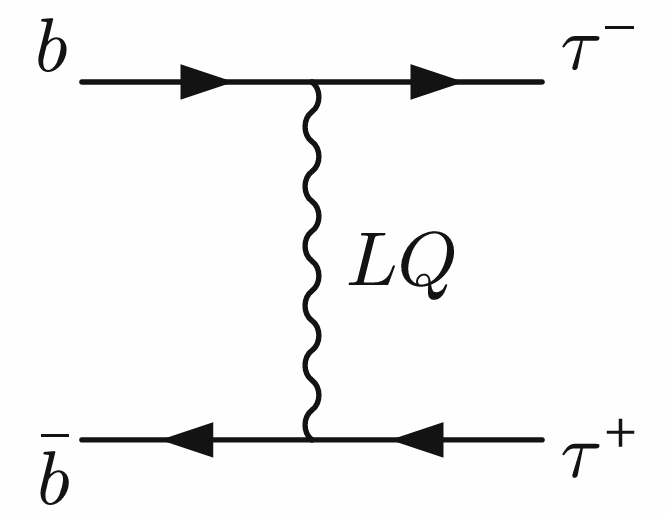
\includegraphics[width=\linewidth]{non_resonant.png}
	\end{minipage}
	\begin{minipage}{.68\linewidth}
		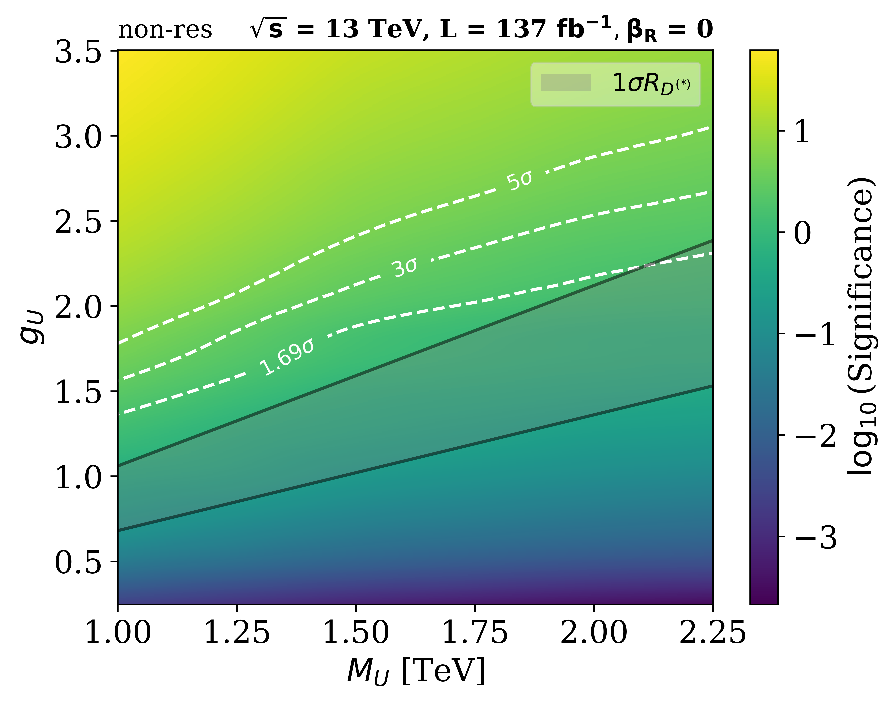
\includegraphics[width=\linewidth]{Significance_Heatmap_13TeV_L137_non-res_combined_woRHC.pdf}
	\end{minipage}

	{\large
		  Non-resonant production is highly dependent on the couplings, so it dominates the regions of high coupling constants at all masses.
	}
\end{frame}

\begin{frame}{Combined Sensitivity Reach}{The Sensitivity Reach / only left-handed currents}
	\begin{center}
		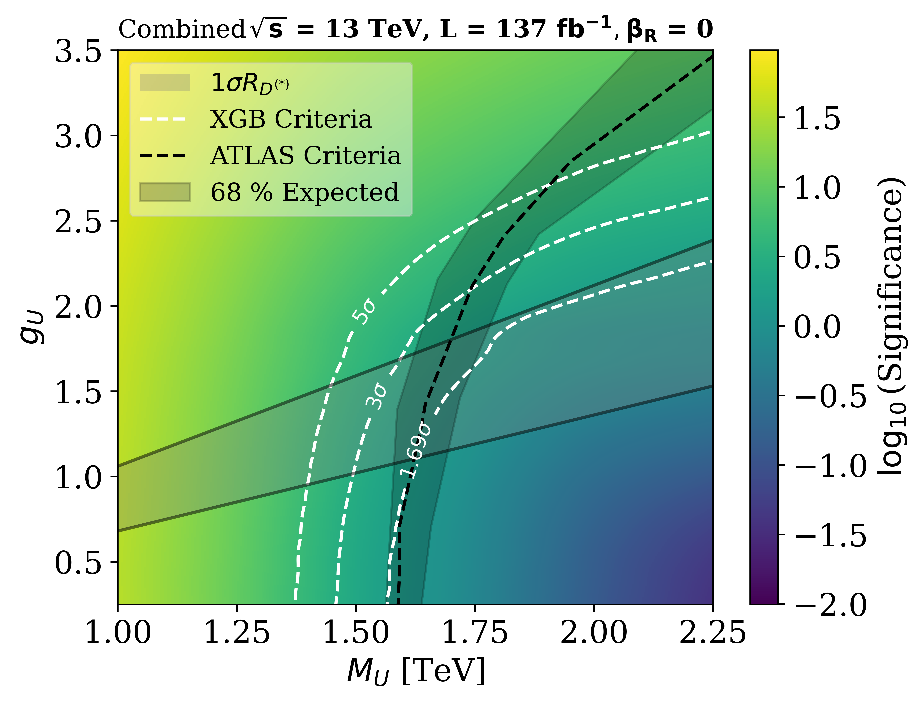
\includegraphics[width=.55\linewidth]{Significance_Heatmap_13TeV_L137_all_combined_woRHC.pdf}
		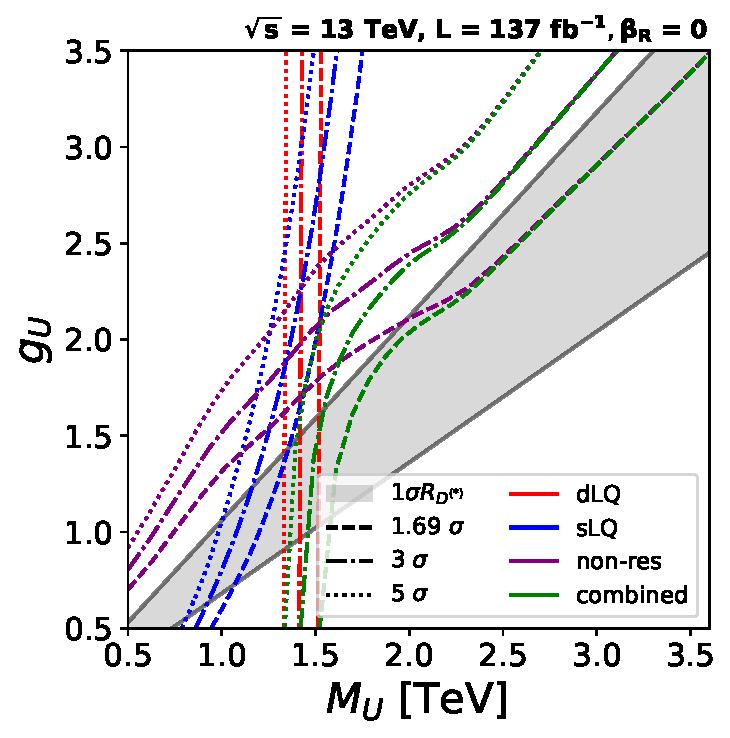
\includegraphics[width=.41\linewidth]{Significance_Curves_13TeV_L137_summary_all_sigmas_woRHC.pdf}
	\end{center}
	{\large
		  The sensitivity of
		all signal production processes combined compares
		our expected exclusion region with the latest one from
		the ATLAS Collaboration [ArXiv:2305.15962], but we suggest better sensitivity for high coupling constants.
	}
	
\end{frame}

\begin{frame}{Combined Sensitivity Reach}{The Sensitivity Reach / only right-handed currents}
	\begin{center}
		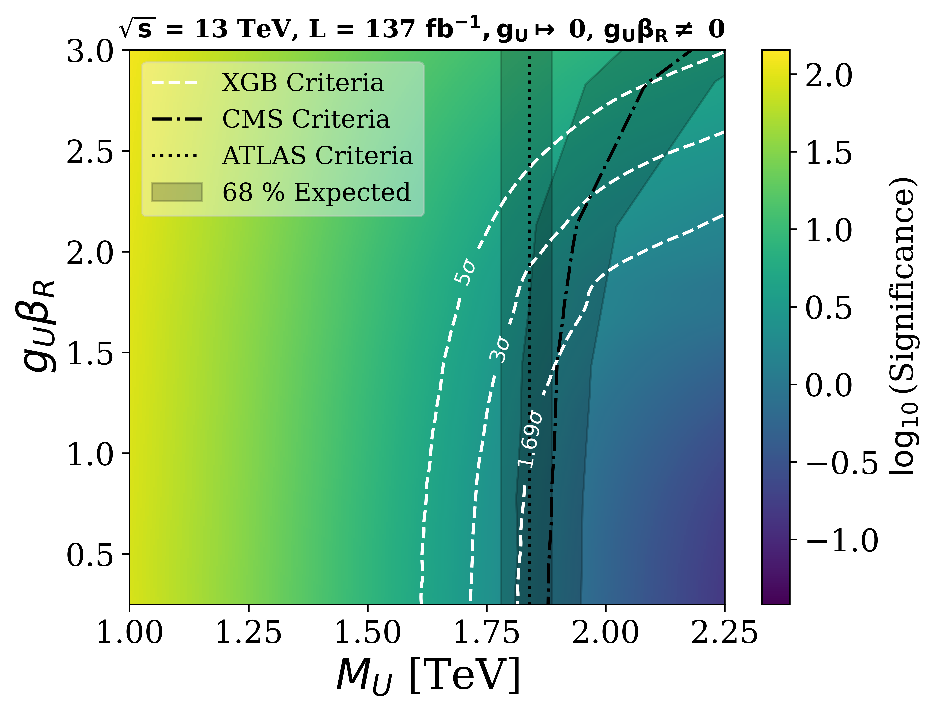
\includegraphics[width=.68\linewidth]{Significance_CMS_Comparison_13TeV_L137_all_combined_woRHC.pdf}
	\end{center}
	{\large
		  The case $BR(lq \rightarrow b \tau) = 1$ corresponds to the only right-handed currents coupling. The sensitivity compared with the latest one from the CMS [2308.07826] and ATLAS Collaborations [2303.01294], again we suggest better sensitivity for high coupling constants.
	}
\end{frame}

\begin{frame}{Combined Sensitivity Reach}{Comparison between different Branching ratios}
	\begin{center}
		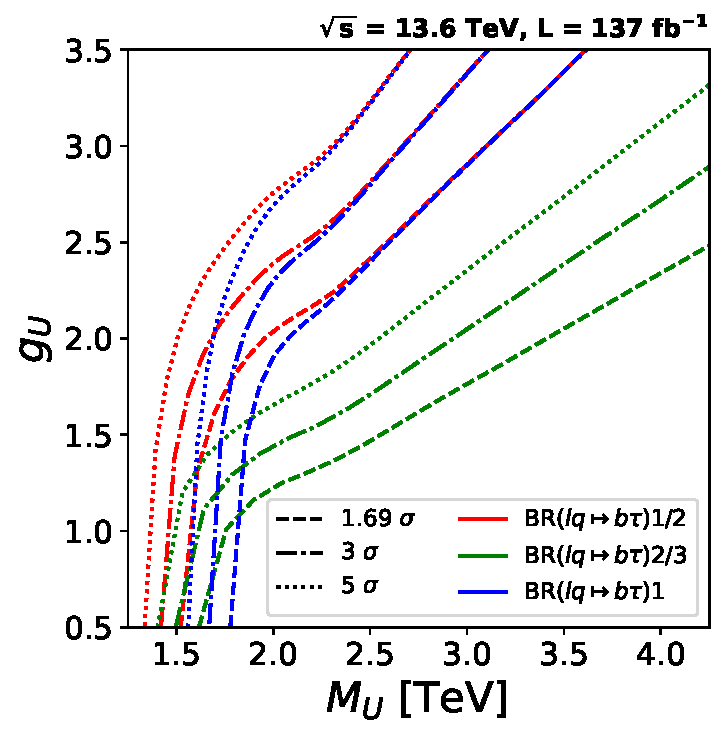
\includegraphics[width=.68\linewidth]{Significance_Curves_Summary_by_BR.pdf}
	\end{center}
\end{frame}

\begin{frame}{Including the $Z'$ boson contribution}{The Sensitivity Reach / only left-handed currents}
	\begin{center}
		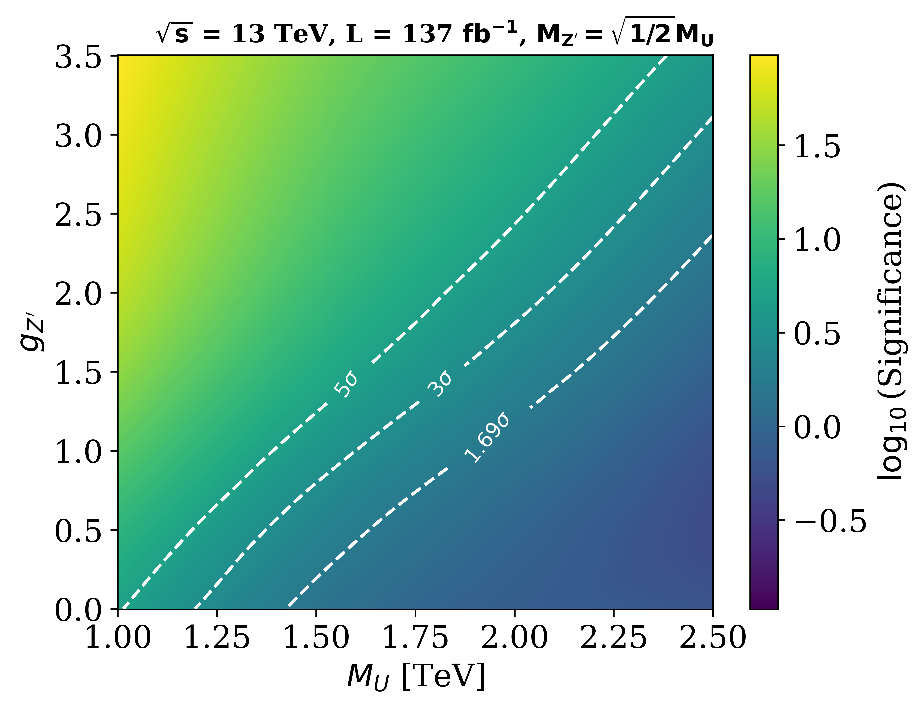
\includegraphics[width=.68\linewidth]{zp_lower_limit_woRHC_gu1_75.pdf}
	\end{center}
	{\large
		  As is expected if the $Z'$ boson is lighter than the leptoquark, the sensitivity is incresed for higher leptquark masses, due to the additional contribution to the cross section.
	}
\end{frame}

\begin{frame}{Including the $Z'$ boson contribution}{The Sensitivity Reach / only left-handed currents}
	\begin{center}
		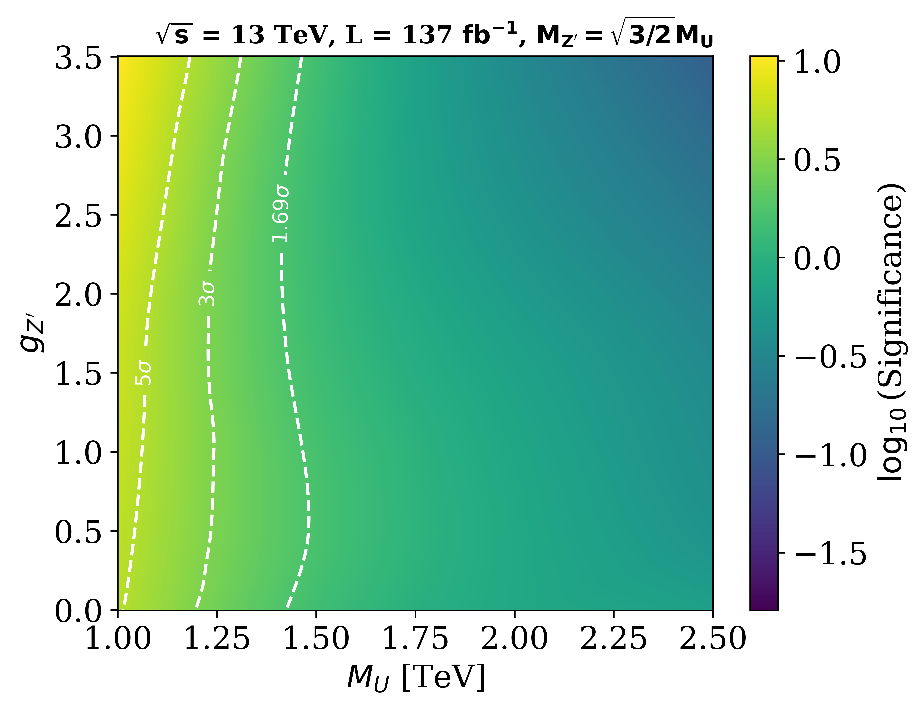
\includegraphics[width=.68\linewidth]{zp_upper_limit_woRHC_gu1_75.pdf}
	\end{center}
	{\large
		  If the $Z'$ boson is heavier than the leptoquark, the sensitivity looks like the one without the $Z'$ boson, except for the region near to the leptoquark coupling constant.
	}
\end{frame}

\begin{frame}{Including the $Z'$ boson contribution}{The Sensitivity Reach / only left-handed currents}
	\begin{center}
		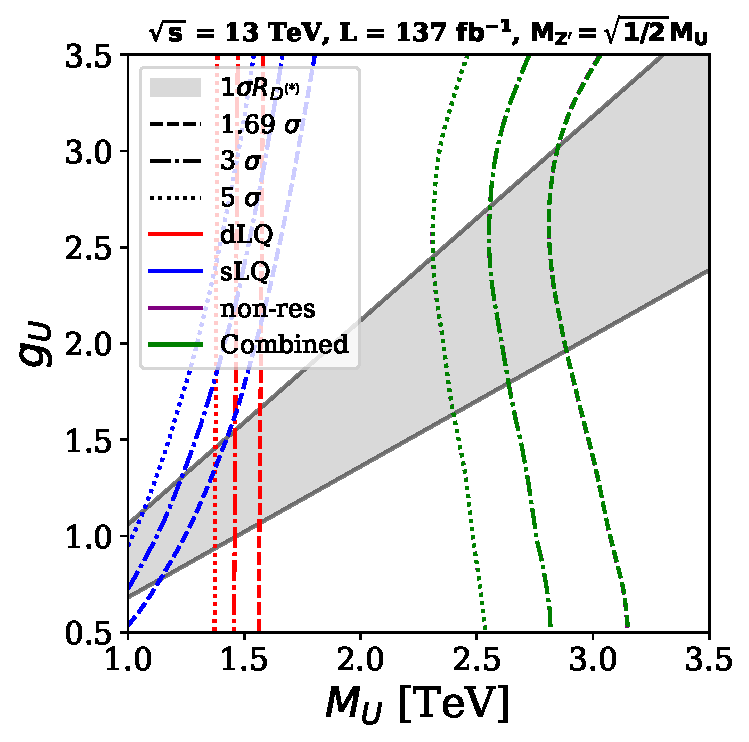
\includegraphics[width=.45\linewidth]{zp_lower_limit.pdf}
		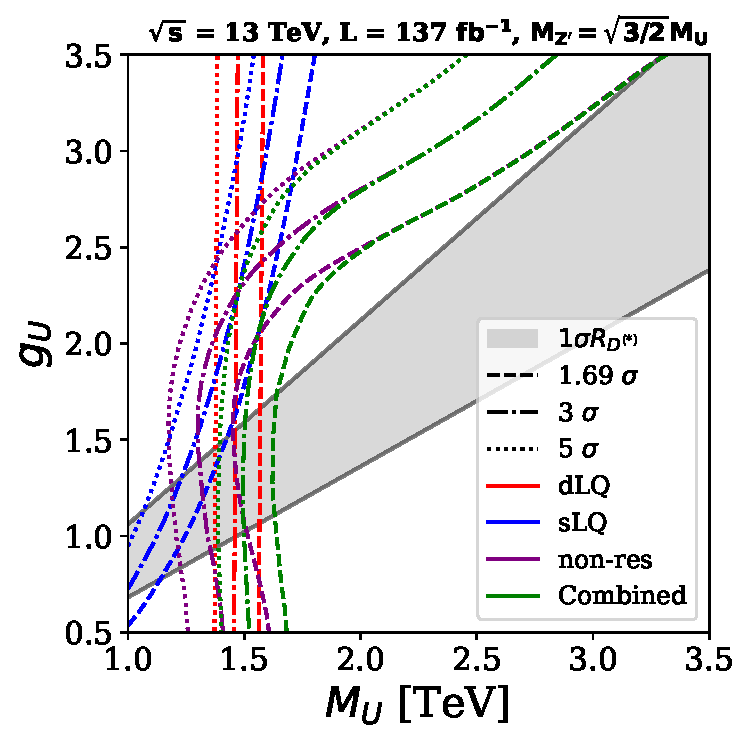
\includegraphics[width=.53\linewidth]{zp_upper_limit.pdf}
	\end{center}
\end{frame}

\begin{frame}{Summary}
	\begin{itemize}
		\item Experimental searches for LQs with preferential couplings to third generation fermions are of great interest due to their potential to explain tensions in the $R(D)$ and $R(D^{*})$ decay ratios of B mesons with respect to SM predictions. \vfill
		
		\item Studies on the production of $U_1$ LQs with preferential couplings to third generation fermions, considering different couplings, masses, and chiral currents performed using $\mathrm{p}\,\mathrm{p}$ collisions at $\sqrt{s} = 13TeV$ and their interferences with a $Z^{\prime}$ boson.  \vfill
		
		\item New computational techniques based on machine learning (ML) as BDTs are important to improve sensitivity to potential signs of physics beyond the SM. \vfill
		
		\item Expected signal significance for sLQ, dLQ, and non-res production, and their combination, presented as contours on a two-dimensional plane of $g_U$ versus $M_U$ for exclusive couplings to left-handed, mixed, and exclusive right-handed currents making enfasis in the region of phase space that could explain B meson anomaly is presented. \vfill

		\item Sensitivity to probe the parameter space is highly dependent on the chirality of the couplings and effects of a companion $Z^{\prime}$ boson on non-res production can significantlyimpact the results. \vfill
		
		\item Non-res production remains an essential channel for probing LQs in the future. \vfill
	\end{itemize}
	
\end{frame}

% \begin{frame}{Current and Future Work}
% 	\begin{itemize}
% 		\item asd
% 	\end{itemize}
	
% \end{frame}

\end{document}

